\documentclass[12pt,a4j,report,dvipdfmx]{jsbook_mod}
\usepackage{url}
\usepackage{amsmath}
\usepackage{graphicx}
\usepackage{fancybox}
\usepackage{eclbkbox}
\usepackage{fancyhdr}
\usepackage{titling}
\usepackage{remreset}
\usepackage{listings}
\usepackage{here}
\usepackage{algorithm}
\usepackage{algorithmic}
\usepackage{tocloft}
\usepackage{txfonts}
\usepackage{listings}
\usepackage{lscape}
%\documentclass{jarticle}
\usepackage{here}
\usepackage{siunitx}
\usepackage{comment}
\usepackage[dvipdfmx]{graphicx}

\lstset{
  basicstyle={\ttfamily},
  identifierstyle={\small},
  commentstyle={\smallitshape},
  keywordstyle={\small\bfseries},
  ndkeywordstyle={\small},
  stringstyle={\small\ttfamily},
  frame={tb},
  breaklines=true,
  columns=[l]{fullflexible},
  numbers=left,
  xrightmargin=0zw,
  xleftmargin=3zw,
  numberstyle={\scriptsize},
  stepnumber=1,
  numbersep=1zw,
  lineskip=-0.5ex
}


%図表目次の頭のため
%図表目次の番号の頭に「図」・「表」と入れるやつここから
\newlength{\mylenfig}%図用
\renewcommand{\cftfigpresnum}{\figurename\enspace}
\renewcommand{\cftfigaftersnum}{\hspace{1em}}
\settowidth{\mylenfig}{\cftfigpresnum\cftfigaftersnum}
\addtolength{\cftfignumwidth}{\mylenfig}

\newlength{\mylentab}%表用
\renewcommand{\cfttabpresnum}{\tablename\enspace}
\renewcommand{\cfttabaftersnum}{\hspace{1em}}
\settowidth{\mylentab}{\cfttabpresnum\cfttabaftersnum}
\addtolength{\cfttabnumwidth}{\mylentab}

\setlength{\cftchapnumwidth}{3.8em}%何故か崩れる章のインデント調節
\setlength{\cftbeforetoctitleskip}{0pt}
\setlength{\cftaftertoctitleskip}{10pt}

\setlength{\cftbeforeloftitleskip}{0pt}
\setlength{\cftafterloftitleskip}{10pt}

\setlength{\cftbeforelottitleskip}{0pt}
\setlength{\cftafterlottitleskip}{10pt}
%図表目次の番号の頭に「図」・「表」と入れるやつここまで
\begin{document}
\pagestyle{empty}
% vim: set filetype=tex :
\title{ 同時送信フラッディングにおける\\ 到達性を考慮したホスト選択手法}

\begin{titlepage}
\renewcommand{\baselinestretch}{1.5}
\begin{center}
{\Large
電気通信大学 情報理工学域 \\
令和元年度 卒業論文 \\
}
\end{center}
\renewcommand{\baselinestretch}{1.0}
{\LARGE
\begin{center}
\mbox{} \\
\fbox{ \begin{tabular}{c}
\thetitle 
\end{tabular} }
\end{center}
\mbox{} \\
\begin{figure}[h]
\begin{center}
\includegraphics[width=0.15 \linewidth,bb=0 0 160 160]{graphs/ueclogo.png}
\end{center}
\end{figure}

\renewcommand{\baselinestretch}{1.5}
\begin{center}
学籍番号 1610109 \\
氏名 榎戸 菜々穂 \\
\mbox{} \\
I\hspace{-.1em}I類 セキュリティ情報学プログラム\\
\mbox{} \\
指導教員    山本 嶺 准教授\\
提出日 令和2年2月6日(木)
\end{center}
}
\end{titlepage}
\renewcommand{\baselinestretch}{1.0}

\newpage
\pagestyle{plain}
\setcounter{page}{1}
\pagenumbering{roman}
% vim: set filetype=tex :

\newcounter{keywordcnt}
\newcommand{\keyword}[1]{\addtocounter{keywordcnt}{1} \underline{\thekeywordcnt . #1} }
{\Large
\begin{center}
卒業論文2019年度(令和元年度) \\
\fbox{ \begin{tabular}{c}
\thetitle
\end{tabular} }
\end{center}
}
\section*{論文要旨}

\indent IoT通信技術の発達に伴って,構造物や工場内のモニタリングにおいて無線センサネットワークを利用した通信を用いるセンシングデータの収集が期待されている.例えば工場では,機器同士の接続は有線が多いが,これを無線に置き換えれば機器の配置換えにかかる作業時間の短縮やコスト削減が期待できる.しかし,高い信頼性が求められる制御系の工場システムにおいては,通信速度や信頼性に対する懸念から,現状,無線化は4\%程度しか進んでいない~\cite{IoT}.このような背景の下,フレーム受信後にバックオフ時間をおかずにブロードキャストを繰り返す同時送信フラッディング(CTF : Concurrent Transmission Flooding)が提案されている.
同時送信フラッディングの性能は,ノード同士の時刻同期の精度に大きく左右されるため,スケジュール機能をもったホストノードが時刻同期を担っている.しかし,ホストノードの配置によっては,ホストノードからの通信を受信できないノードが発生し,ネットワーク分断が発生する可能性がある.
そこで,本研究ではホストノードから他ノードへの到達性を考慮したホスト選択手法を提案することでネットワーク分断を減らし,同時送信フラッディングの性能向上を目指す.
具体的には,ネットワーク指標によってホスト適性が高いノードを選んだ場合の最短経路長の平均や分布,ネットワーク分断のをシミュレーションによって評価した.
その結果,従来手法よりも最短経路長平均とネットワーク分断の発生確率が改善されることが分かった.また,媒介中心性によるホスト選択が同時送信フラッディングに適していることが分かった.今後の課題としては,本研究において検討しなかったネットワーク指標におけるホスト選択が同時送信フラッディングに与える影響の評価,及び実機や実際の電波伝搬を考慮したシミュレーションによる検討等があげられる.

%あと結果と課題

\vspace{-5mm}

\section*{キーワード}\vspace{-3mm}
\keyword{同時送信フラッディング}
\keyword{ZigBee}
\keyword{CTF}
\keyword{マルチホップ}
\keyword{ネットワーク中心性}
\keyword{ダイクストラ法}



\thispagestyle{fancy}
\renewcommand{\headrulewidth}{0.0pt}
\rfoot{\vspace{-5zh}電気通信大学 情報理工学域 I\hspace{-.1em}I類 セキュリティ情報学プログラム \\ \LARGE{榎戸 菜々穂}}

\newpage
\setcounter{tocdepth}{2}
\tableofcontents
\newpage
\listoffigures
\newpage
\listoftables
\newpage
\setcounter{page}{1}
\pagenumbering{arabic}


\chapter{背景と目的}

\section{研究背景}
近年,モノとモノをネットワークでつなぐことで得られるデータをモニタリングや異常検知に活用するIoT(Internet of Things)が注目されている.
IoT活用による利益は,工場分野などを中心に最大で約1300兆円にも上ると推定されている~\cite{IoT}.IoT技術の成長を支えるのは,安価で小さなセンサとそれらのデータのやり取りを可能とする無線通信技術である.
無線通信規格の一つであるZigBee~\cite{zigbee}はIoT機器によく用いられる.通信距離はおよそ30-50\si{\metre}と短いが,個々が中継局としての機能をもつため,マルチホップ通信により従来は届かなかった場所や広範囲への通信が可能である.


しかし,低遅延・高信頼な通信という点で無線通信には課題が多い.工場や製造分野ではIoT技術の活用による高い経済効果が想定されているにもかかわらず,工場内の通信方式にしめる無線通信の割合は4\%程度である~\cite{IoT}.
これは,工場内で多くの様々な機器が作動しているためである.無線通信では,複数の送信元からの電波が受信端末側で干渉した場合,受信端末がパケットの受信に失敗する.多くの機器が無線通信を行う工場では電波が干渉する可能性が高まるため,一般的に損失率は上昇する.また,機器が再送を繰り返した場合,遅延が増加する.

この問題に対し,同時送信フラッディングと呼ばれる転送方法が提案されている.
同時送信フラッディングは,一般に無線通信において性能劣化となる干渉を有効的に活用することで,受信成功率改善する手法である.
これは,干渉が起きた場合でも受信ノードにおける各送信ノードからの電波到来時間差が0.5\si{\micro\second}以内であれば復調が可能であるという発見を利用した技術である.本論文では,以後,復調が可能である干渉を建設的干渉,それ以外を破壊的干渉という.同時送信フラッディングは,ノードの時刻同期ができていれば細かい制御を必要とせずにフラッディングのみでデータをネットワーク全体に転送できる.同時送信フラッディングは2011年にFerrariらによって提唱され,2017年にソナス株式会社がUNISONetとして実用化した.具体的には橋梁での地震モニタリング,製造設備の予防保全等のための振動計測,農場での植物生育モニタリング等に活用されている~\cite{sonas}.

同時送信フラッディングがモニタリングに適している理由として,
\begin{itemize}
    \item ルーチングレスな技術でありネットワークの知識のない人であっても扱いやすいこと
    \item サンプリングタイミングを同期させているため得られたデータの解析が容易
    \item 高信頼・低遅延な通信
\end{itemize}
などがある.

同時送信フラッディングの性能は受信端末側へのパケット到達タイミングに大きく左右される.パケット到達タイミングの調整にはノード間の時刻同期が必須であり,スケジュール機能を持ったホストノードがその管理を担っている.そのため,ホストノードに障害が発生した場合,建設的干渉ではなく,破壊的干渉が生じる可能性が高い.そのため,より安定的な転送制御を実現するためには,ホストノードの耐障害性を向上させるための対策が必要である.
ホスト障害対策として先行研究~\cite{lowpower}では,全ノードがホストノードの機能をもつことで,ホストノードが故障や通信できない状態に陥っても,別のノードにフェイルオーバし、ホストノードの耐障害性を向上させていた.
ここでの新たなホストノードの選出方法は,あらかじめ全ノードが保持しているリストをラウンドロビン方式で参照するものであった.なお,リスト内にはホストノードに対応したチャネルが指定されておりホストノードの変更に伴い,転送を行うチャネルも切替わる.

\section{研究目的}
前述のように,従来手法ではリストに基づくホスト選出を行っており,決められた時間内に新ホストからのパケットを受信できなかったノードが,チャネルを切替え続けてメインのネットワークに合流できず,ネットワーク分断が生じる可能性があった.本研究では,特定のホストノードに障害が発生した場合においても,高い信頼性を維持したまま同時送信フラッディングによる転送を継続するため,到達性を考慮してホストノードを決定する手法を提案する.ここで到達性は,後述の最短経路長平均やInf数を意味する.ネットワーク上におけるノードの重要性を評価するための指標である次数中心性や媒介中心性などのネットワーク指標が高いノードをホストノードとすることで,同時送信フラッディングにおける信頼性の向上を目指す.%同時送信フラッディングにおける到達性にどのように影響するかを評価する.

ホストノードを上記のネットワーク指標で選出し,限定することで従来のラウンドロビン方式のホスト選出と比較して,最短経路長やホストノードからのスケジューリングパケットが到達しないノードが減るのではないかと考えた.その結果,ネットワーク分断や遅延が減り,同時送信フラッディングの信頼性向上が期待できる.

\section{本論文の構成}
本論文の構成は以下の通りである.
\begin{itemize}
\item{第1章 ワイヤレスセンサーネットワーク分野の背景と目的}
\item{第2章 同時送信フラッディング}
\item{第3章 到達性を考慮したホスト選択手法}
\item{第4章 性能評価}
\item{第5章 結論と今後の課題}
\end{itemize}

第2章では同時送信フラッディングやマルチホップネットワークで使われる既存技術や関連研究について述べる.第3章では同時送信フラッディングにおけるホスト選択の提案手法について述べ,第4章ではシミュレーションプログラムの詳細とそれによる提案手法の評価結果を示す.第5章では本研究で得られた結果に基づく結論と,今後の課題について述べる.

本論文における約束事は以下のとおりである.
\begin{itemize}
    \item 章,節は例のような順序で大項目から小項目へと移る. (例: 第2章,2.1)
    \item 式,図,及び表は,章単位で通し番号をつける. (例: 図 3.2)
    \item 参考文献は,文章中及び文章の末尾に文献番号で示す.
\end{itemize}


\chapter{同時送信フラッディング}

\section{マルチホップネットワークの特徴}
マルチホップとはノードからノードへバケツリレーのようにデータを転送していく方法である.マルチホップネットワークは,ノードが中継することによって直接波では届かない場所までデータを届けることができるという特徴がある.
全てのノードが受信/送信両方を行い,中継を繰り返すことでネットワーク全域にデータを広める.具体的には,送られてきたデータに対して受け取ったノードが,データの目的地に応じて送り出す経路を変える.これをルーチングという.このルーチングをどのように決めるのか・行うのかの決まり事がルーチングプロトコルである.ルーチングプロトコルはさまざまなものが考案されているが,大きく二つにわけられる.

\begin{itemize}
    \item プロアクティブ型 端末間で常に情報をやり取りし,経路表を更新し続ける方法(ex.OLSR)
    \item リアクティブ型 端末からの要求があった時にのみ経路表の更新を行う方法(ex.AODV,ZigBeeもAODVべース)
\end{itemize}
従来のマルチホップ通信は干渉を通信品質を下げるものとして捉え,複雑なルーチングプロトコルによって干渉を避けることに焦点を当てていたが,同時送信フラッディングは送信タイミングの調整によって干渉による影響を復調が可能な範囲内に抑えること,マルチパスにすることで成功確率を上げることに焦点を当てている.
また,同時送信フラッディングは,各ノードが経路情報を持たずにフラッディングのみで転送を行い,ルーチングを考えない.ノードが互いの通信状態について関知しないという点で従来のマルチホップ通信と異なる.
つまり,同時送信フラッディングでは,ルーチングを廃したフラッディングによるデータ転送を行っている同時送信フラッディングでのデータ転送は基本的にマルチパス転送であり,ユニキャスト通信において用いられるバックオフ時間が不要である.このことから,高信頼かつ低遅延な通信を実現可能である.

\section{同時送信フラッディング概要}
同時送信フラッディングは2011年に提唱されたZigBeeにおけるマルチホッププロトコルの一つである.
同時送信フラッディングの主な特徴は,建設的干渉と時刻同期である.ここで,建設的干渉とは,空間や時間,周波数が同一の信号を送出した場合においても,元のデータが復調可能である現象であり,受信ノードにおける各送信ノードからの電波到来時間差が0.5\si{\micro\second}以内に収まる場合に発生すると述べられている\cite{Effi}.その後の研究で建設的干渉が起きる場合もあれば起きない場合もあることがわかり,データの復調の成功が建設的干渉によるものなのかマルチパスによるものなのか厳密に区別した評価は行われていない\cite{revising}.しかし,受信ノードにおける各送信ノードからの電波到来時間差が0.5\si{\micro\second}以内に収まる場合に高い成功率を実現していることは事実である.
また,この0.5\si{\micro\second}は,実験から得られた値である.この値はZigBee\cite{zigbee}の変調方式に関係している.詳しくは\ref{sec:modulation}章で述べる.
また,受信ノードにおける各送信ノードからの電波到来時間差を0.5\si{\micro\second}以内に収めるためには,ノード間の正確な時刻同期が必要である.これはパケットに含まれる中継カウンタと伝送時間の計算から,Initiatorと転送ノードを相対的に時刻同期することで実現している.詳しくは\ref{sec:time}章で述べる.

 また,同時送信フラッディングは,従来の転送手法と比較して信頼性が高く,部分的な通信障害やノードの障害が同時送信フラッディングの転送性能に与える影響がわずかであることが実験によって実証されている.先行研究\cite{lowper}によると,Wi-Fi干渉による通信障害に対して平均99\%以上のデータ収集率を示し,デューティ比も低い値を維持している.ここでいうデューティ比とは,起動時間に占める送信時間の割合のことで,この値が大きいということは再送が多いということを意味する.
 ノード障害においても,既存のプロトコルDozerがデータ収集率を96\%に落としたのに対し,同時送信フラッディングを用いたプロトコルによる通信は常時99\%以上の安定したデータ収集率を示している.

\section{ZigBeeについて}
\label{sec:modulation}
ZigBeeにおける物理層とMAC層は,IEEE802.15.4規格を適用している.IEEE802.15.4規格では拡散方式がDSSS(Direct Sequence Spread Spectrum),変調方式がO-QPSK(Offset-Quaternary Phase Shift Keying)である.ZigBeeのプロトコルスタックを図\ref{fig:stack}に示す.本研究の焦点はホストノードの選び方が同時送信フラッディングに及ぼす影響だが,同時送信フラッディングの原理がZigBeeの変調方式に根差しているため軽く触れておく.

\begin{figure}[H]
  \centering
  \includegraphics[width=0.3\textwidth]{figures/prostack.pdf}
  \caption{ZigBeeのプロトコルスタック}
  \label{fig:stack}
\end{figure}
%https://www.oki.com/jp/Home/JIS/Books/KENKAI/n200/pdf/200_R19.pdf


DSSSでは信号を4ビットごとに分け,そのかたまりを16パターンのシンボルにマッピングする.これをさらに32ビットの疑似ランダムノイズ(PN)符号(これをチップという)と掛け合わせて広い帯域に拡散させる.すると図\ref{fig:DSSS1}に示すように信号は広帯域に広がり,出力が下がる.復調は逆の手順で行われる.信号を広帯域に拡散させることの利点は,出力が下がることで信号が互いに干渉しづらくなることである.また,突発的なノイズや妨害は図\ref{fig:DSSS2}に示すように復調の過程で拡散され,影響が少なくなるため耐性がある.
O-QPSK(Offset-QPSK)は0と1の二値信号でデータを伝送するデジタル変調方式の一種である.基準信号を位相変調するのがPSKで,4段階で位相の変調を行うのがQPSKである.O-QPSK(Offset-QPSK)は先述のシンボルを,奇数シンボル(Qデータ)と偶数シンボル(Iデータ)間で$\pi$/2に相当する時間分ずらして送信する方法である.信号成分の振幅と位相は極座標において半径と位相で表されるが,これを極座標系から直交(X,Y)座標系に変換したものがQ/Iデータである.
この$\pi$/2差を得るために同位相Qチップは,逆位相Iチップに対してTc=0.5\si{\micro\second}だけ遅延される~\cite{Effi}.

\begin{figure}[H]
  \centering
  \includegraphics[width=0.8\textwidth]{figures/6.pdf}
    \vspace{-40mm}
  \caption{DSSS拡散によって元信号の周波数帯が広がる様子}
  \label{fig:DSSS1}
\end{figure}

\begin{figure}[H]
  \centering
  \includegraphics[width=0.8\textwidth]{figures/7.pdf}
  \vspace{-50mm}
  \caption{復調におけるノイズ処理}
  \label{fig:DSSS2}
\end{figure}
%https://ascii.jp/elem/000/000/462/462443/

\section{同時送信フラッディング詳細}
以下の図\ref{fig:ctf_ju}は同時送信フラッディングのフローチャートである.フローチャートにおいてはフローチャート上で隣り合うノード同士が通信可能とする.また,ホストノードやInitiatorとノード1,2,3は同じハードウェアであり,状況に応じて役割を変更している.今回はホスト障害後にnode1が新ホスト,Initiator同じノードが続行するという状況をフローチャートに示した.加えて,中継カウンタ(c=i)が同じ転送は,フローチャート上で,仕様上タイミングがずれて見えるが,実際は同じ時間に送信されていると見なす.また,フローチャート上の赤いライフラインは,ノードが電源をonにして待機している状態,白いライフラインはノードが転送中であることを示している.図\ref{fig:ctf_ov}は同時送信フラッディングを別の形で示したものである.緑色のノードはフローチャートにおいてライフラインがない状態,グレーのノードがフローチャートにおける赤いライフラインを示している.
フローチャートとノード図の対応を表\ref{tab:taio}に示す.

\begin{table}[H]
  \caption{対応表}
  \begin{tabular}{c|c} \hline \hline
     フローチャート& ノード図  \\\hline
     host&ホストノード(赤)\\
    Initiator&上段〇1の黄色ノード,下段〇1の黄色ノード\\
    node1,2,3&上記2つ以外のノード\\\hline
     ライフラインなし & 休眠ノード(緑)\\
     赤いライフライン & 受信待機ノード(灰色)\\
     白いライフライン & 青い円内の灰色ノード\\\hline\hline
  \end{tabular}
  \label{tab:taio}
\end{table}

同時送信フラッディングはスケジューリングフェーズとデータ転送フェーズにわかれる.
図\ref{fig:ctf_ju}においては赤いコメントでスケジューリングフェーズと転送フェーズの区切りを示している.
(1)図\ref{fig:ctf_ov}における最初のスケジューリングフェーズ(図\ref{fig:ctf_ov}だと〇0)\\
ホストノードからその他のノードにスケジュールパケットを送り,時刻同期(詳しくは\ref{sec:time}章で述べる)とノードの生存確認及びノード間の通信確認を行うフェーズである.全ノードとやり取りが済むと転送フェーズに移る.\\

(2)図\ref{fig:ctf_ov}における最初の転送フェーズ(図\ref{fig:ctf_ov}だと上段の〇1-4)\\
Initiatorが最初の送信を行い,Initiatorからの信号の到達範囲(青い円)内のノードがパケットを受信する.パケットを受信したノード(Receiver)は受信後即座に転送を行い転送ノードとしての役割を果たす.また1フェーズにおける転送回数が設定されていて,その上限に達したノードは,転送後電源をoffにする(図\ref{fig:ctf_ov}だと緑の丸の休眠ノード).理論上はホップ数$\times$伝送時間で図\ref{fig:ctf_ov}〇4の状態(ネットワークにデータが行き渡った状態)になる.\\

(3)二回目以降の転送フェーズ(図\ref{fig:ctf_ov}だと下段の〇1-4)\\
スケジューリングフェーズの段階で休眠後最初に目覚めるノード(Initiator)が指定されている.Initiatorが目覚める時間は直前の転送フェーズが終わった直後なので,ホップ数$\times$伝送時間で大体見当がつく.Initiator以外のノードはスケジューリングフェーズでInitiatorに対して相対的に時刻同期が行われているため,そこから逆算してデータが送られてくる直前に電源をonにし,転送後即座にoffにすることができる.転送を行うとき以外は電源をoffにしているため省電力である.

\vspace{-30mm}
\begin{figure}[H]
  \centering
  \includegraphics[width=1\textwidth]{figures/sequence_jurai.eps}
  \caption{同時送信フラッディングの従来フローチャート}
  \label{fig:ctf_ju}
\end{figure}

 \begin{figure}[H]
\centering
\includegraphics[width=0.85\textwidth]{figures/newctf.pdf}
 \vspace{-1mm}
 \caption{同時送信フラッディング概要}
 \label{fig:ctf_ov}
\end{figure}

同時送信フラッディングの参加ノードは,全てのノードが状況に応じてホスト,Initiator,Receiverの役割を担う~\cite{Effi}.Initiatorは,フラッディング開始時に最初の送信を行うノードである.
Reciverは,データが届いたことを検知した直後,即座に転送するノードである.Receiverのイベントのトリガーは無線信号である.Receiverはデータ受信後即座にデータを転送する.このように状況に応じて各ノードが適した役割を担い,マルチホップでデータをネットワーク内に拡散している.
Receiverのトリガーは無線信号の受信であるが,最初の送信を行うInitiatorはホストノードから受け取ったスケジュールにしたがって指定された時間に送信を開始する.転送フェーズが終了し全てのノードが電源offにしても,Initiatorは指定時間に電源をonにする.Initiator以外のノードはInitiatorに対し,相対的に時刻同期しているため,Initiatorの復帰時間から逆算して自分の復帰時間を知ることができる.詳しくは\ref{sec:time}で述べる.
また,永遠に転送が続くことを回避するため,あらかじめ決められた一定回数の転送を終えたノードは電源を切って待機する.図\ref{fig:ctf_ov}は転送回数を1回,図\ref{fig:ctf_ju}は転送回数を2回としたときである.

\section{ホスト障害時の動作}

通信障害とノード障害が同時送信フラッディングに与える影響が少ないことは先で述べたが,同時送信フラッディングの管理を担うホストノードに障害が起きると時刻同期とスケジューリングができなくなり支障が出る.既存研究~\cite{lowpower}では,全ノードにスケジューラを配置し,状況に応じてスケジューラの無効/有効を切替えることで,ホストノードが正常に動作しなくなった場合に次のホストノードを選出し,障害に対応している.また,同一チャネル上に複数ホストノードが同時に存在することを回避するため,あらかじめ各ノードがチャネルと一対一対応のホストリストを保持している.

次に同時送信フラッディングのホスト障害時の動作について述べる.図\ref{fig:ctf_ju}においては,赤いノートの二つ目のスケジューリングフェーズと新ホストでのスケジューリングフェーズと最後の拡散フェーズがホスト障害時の動作に該当する.
 
 \begin{itemize}
    \item 待ち時間内にホストノードからのスケジュールパケットが到着しないことで障害検知(図\ref{fig:ctf_ju}:二つ目のスケジューリングフェーズ,図\ref{fig:host1})
    \item リストを参照し,次のチャネルに切替える(図\ref{fig:host2})
    \item チャネルと一対一対応のホストノードが自分かどうか判断
    \item 自分が指定されたノードならホストノードに,でなければ待機(図\ref{fig:host3})
    \item 新ホストがスケジュールパケットを配布(図\ref{fig:ctf_ju},新ホストでのスケジューリングフェーズ)
    \item 新ホストに指定されたInitiatorが最初の送信を行い拡散フェーズ開始(図\ref{fig:ctf_ju},最後の拡散フェーズ)
\end{itemize}

 \begin{figure}[H]
\centering
\includegraphics[width=0.8\textwidth]{figures/host1.pdf}
 \caption{ホスト障害1}
 \label{fig:host1}
\end{figure}

 \begin{figure}[H]
\centering
\includegraphics[width=0.8\textwidth]{figures/host2.pdf}
 \caption{ホスト障害2}
 \label{fig:host2}
\end{figure}

 \begin{figure}[H]
\centering
\includegraphics[width=0.8\textwidth]{figures/host3.pdf}
 \caption{ホスト障害3}
 \label{fig:host3}
\end{figure}

図\ref{fig:host1}に示すように,各ノードが一定時間$T_{hf}$内に現在のホストノードからパケットを受信せず,障害発生を認識すると,リストを参照し次のチャネルに切替える.
このとき,自ノードがリストで指定されている場合,ホストノードとして動作する.チャネル切替後に一定時間経過しても新ホストからのパケットを受信できない場合,再度チャネルを切替える.このように,各ノードがホストノードの通信の有無によりホストノードの生存確認を行うことで,通信環境に応じたホスト選択を可能にしている.一方,この従来手法では,何らかの要因で待ち時間$T_{hf}$以内に新ホストノードからの通信を受信できないことが繰り返された場合,ノードがチャネルを切替え続け,正常に新ホストからの通信を受信したノードと合流できず,ネットワークが分断される可能性がある.



 \section{同時送信フラッディング時刻同期}
 \label{sec:time}
次にノード間の時刻同期について述べる.まず,パケットには中継カウンタcが含まれている.ノードはカウンタを1増やしてからパケットを転送する.そのためノードは中継カウンタの値からそのパケットが何回転送されたものか判別できる.また,ノードはデータ受信時にタイムスタンプを記録しており,カウンタcとc+1のパケットの送信開始時間差$T_{slot}$を推定することができる(図\ref{fig:time}).

\begin{figure}[H]
\centering
\includegraphics[width=0.9\textwidth]{figures/ts.pdf}
 \vspace{-40mm}
 \caption{Initiatorに対する相対的な時刻同期}
 \label{fig:time}
\end{figure}

同時送信フラッディングでは,従来用いられていた,干渉を避けるため一定時間送信を待つというランダムバックオフが不要なため,受信後即座に転送を行う.そのため理論上では,以下の式\ref{ts}でiホップ目のノードの送信開始時間を表せる.なお,$T_i$はカウンタiのパケットの送信開始時間,$T_{ini}$はInitiatorの基準時間である.
\begin{equation}
\label{ts}
T_i=T_{ini}+c・T_{slot}
\end{equation}

実際にはソフトウェア遅延やハードウェアの違いも考慮した時刻同期が必要で~\cite{Effi}では考慮されているが本研究では簡単のため考慮しない.ここで重要なのは,Initiatorの基準時間とパケット内の中継カウンタから,自分の転送開始時刻がわかること,また自身が保持している時間とパケットの中継カウンタから求まるInitiatorの基準時間を比較すれば,自分が転送に参加すべきかどうかが判断できるという点である.



\section{関連研究}
同時送信フラッディングをセンシング基盤Chocoに実装し,実際に10~70台のセンサノードを用いて,橋梁でのモニタリングに適用した先行研究~\cite{monitoring}においては,「ノードの移動に頑健である」「ネットワークに関する専門的な知識が少なくても構築が容易で利用しやすい」という同時送信フラッディングの有意性が確認されている.

\subsection*{LoRaへの適用}
また,物理層プロトコルLoRaと同時送信フラッディングを組み合わせについて検討し,送信時に意図的に遅延を挟むことでパケットエラー率の抑制を図るオフセットCT法が検討されている~\cite{LoRa}.ここから複数の信号を受信した際,信号間の電力差が小さい場合でも同時送信フラッディングにおいては復調が可能であること,遅延をはさんで送信時間をずらすことでさらに正しく復調できる確率が上がることがわかっている.またホップ数の増加に伴う遅延の拡大を抑制できることも確認されている.オフセットCT法は従来のCT法が苦手とするノードが密集している状況においてPRRを大幅に改善することができる.

\subsection*{トラヒック要求に応じたスケジュール割り当て}
また同時送信フラッディングにおいて,各サービスのトラヒック要求に応じて,スケジュール割り当てを行う試みも行われている~\cite{monitoring}.これにより,トラヒック要求がないときはスリープ,トラヒック要求が多いときは優先的にスロット割り当てを行うことができ,消費電力やデータ収集の点から高効率である.


\chapter{到達性を考慮したホスト選択手法}

前述のように,従来手法ではリストに基づくホスト選出を行っていた.待ち時間内に新ホストからのパケットを受信できなかったノードが,メインのネットワークに合流できず,ネットワーク分断が生じる可能性があった.本研究では,より安定的な転送制御を実現するために,到達性を考慮したホスト選択手法を提案する.提案するホスト選択手法を用いた同時送信フラッディングのフローチャートを図\ref{fig:ctf_te}に示す.
ここで到達性を考慮したホスト選択手法とは,媒介中心性と次数中心性によるホスト選択である.これらの算出にはネットワーク全体の隣接行列が既知であることが前提であり,トポロジー情報を保持しない従来の同時送信フラッディングにおいては適用できない.しかし,本研究では,事前のメッセージ交換等により隣接情報を取得しているものとする.そのため,センサノードの位置や距離が既知であり,ノードの位置変更もないという前提でシミュレーションを行う.また,先行研究~\cite{LoRa}の実験によって290\si{\meter}$\times$195\si{\meter}の範囲内ではノードの粗密に関わらず同時送信フラッディングの有効性が確認されているため,ノードの配置範囲を250\si{\meter}四方とした.

\begin{figure}[H]
  \centering
  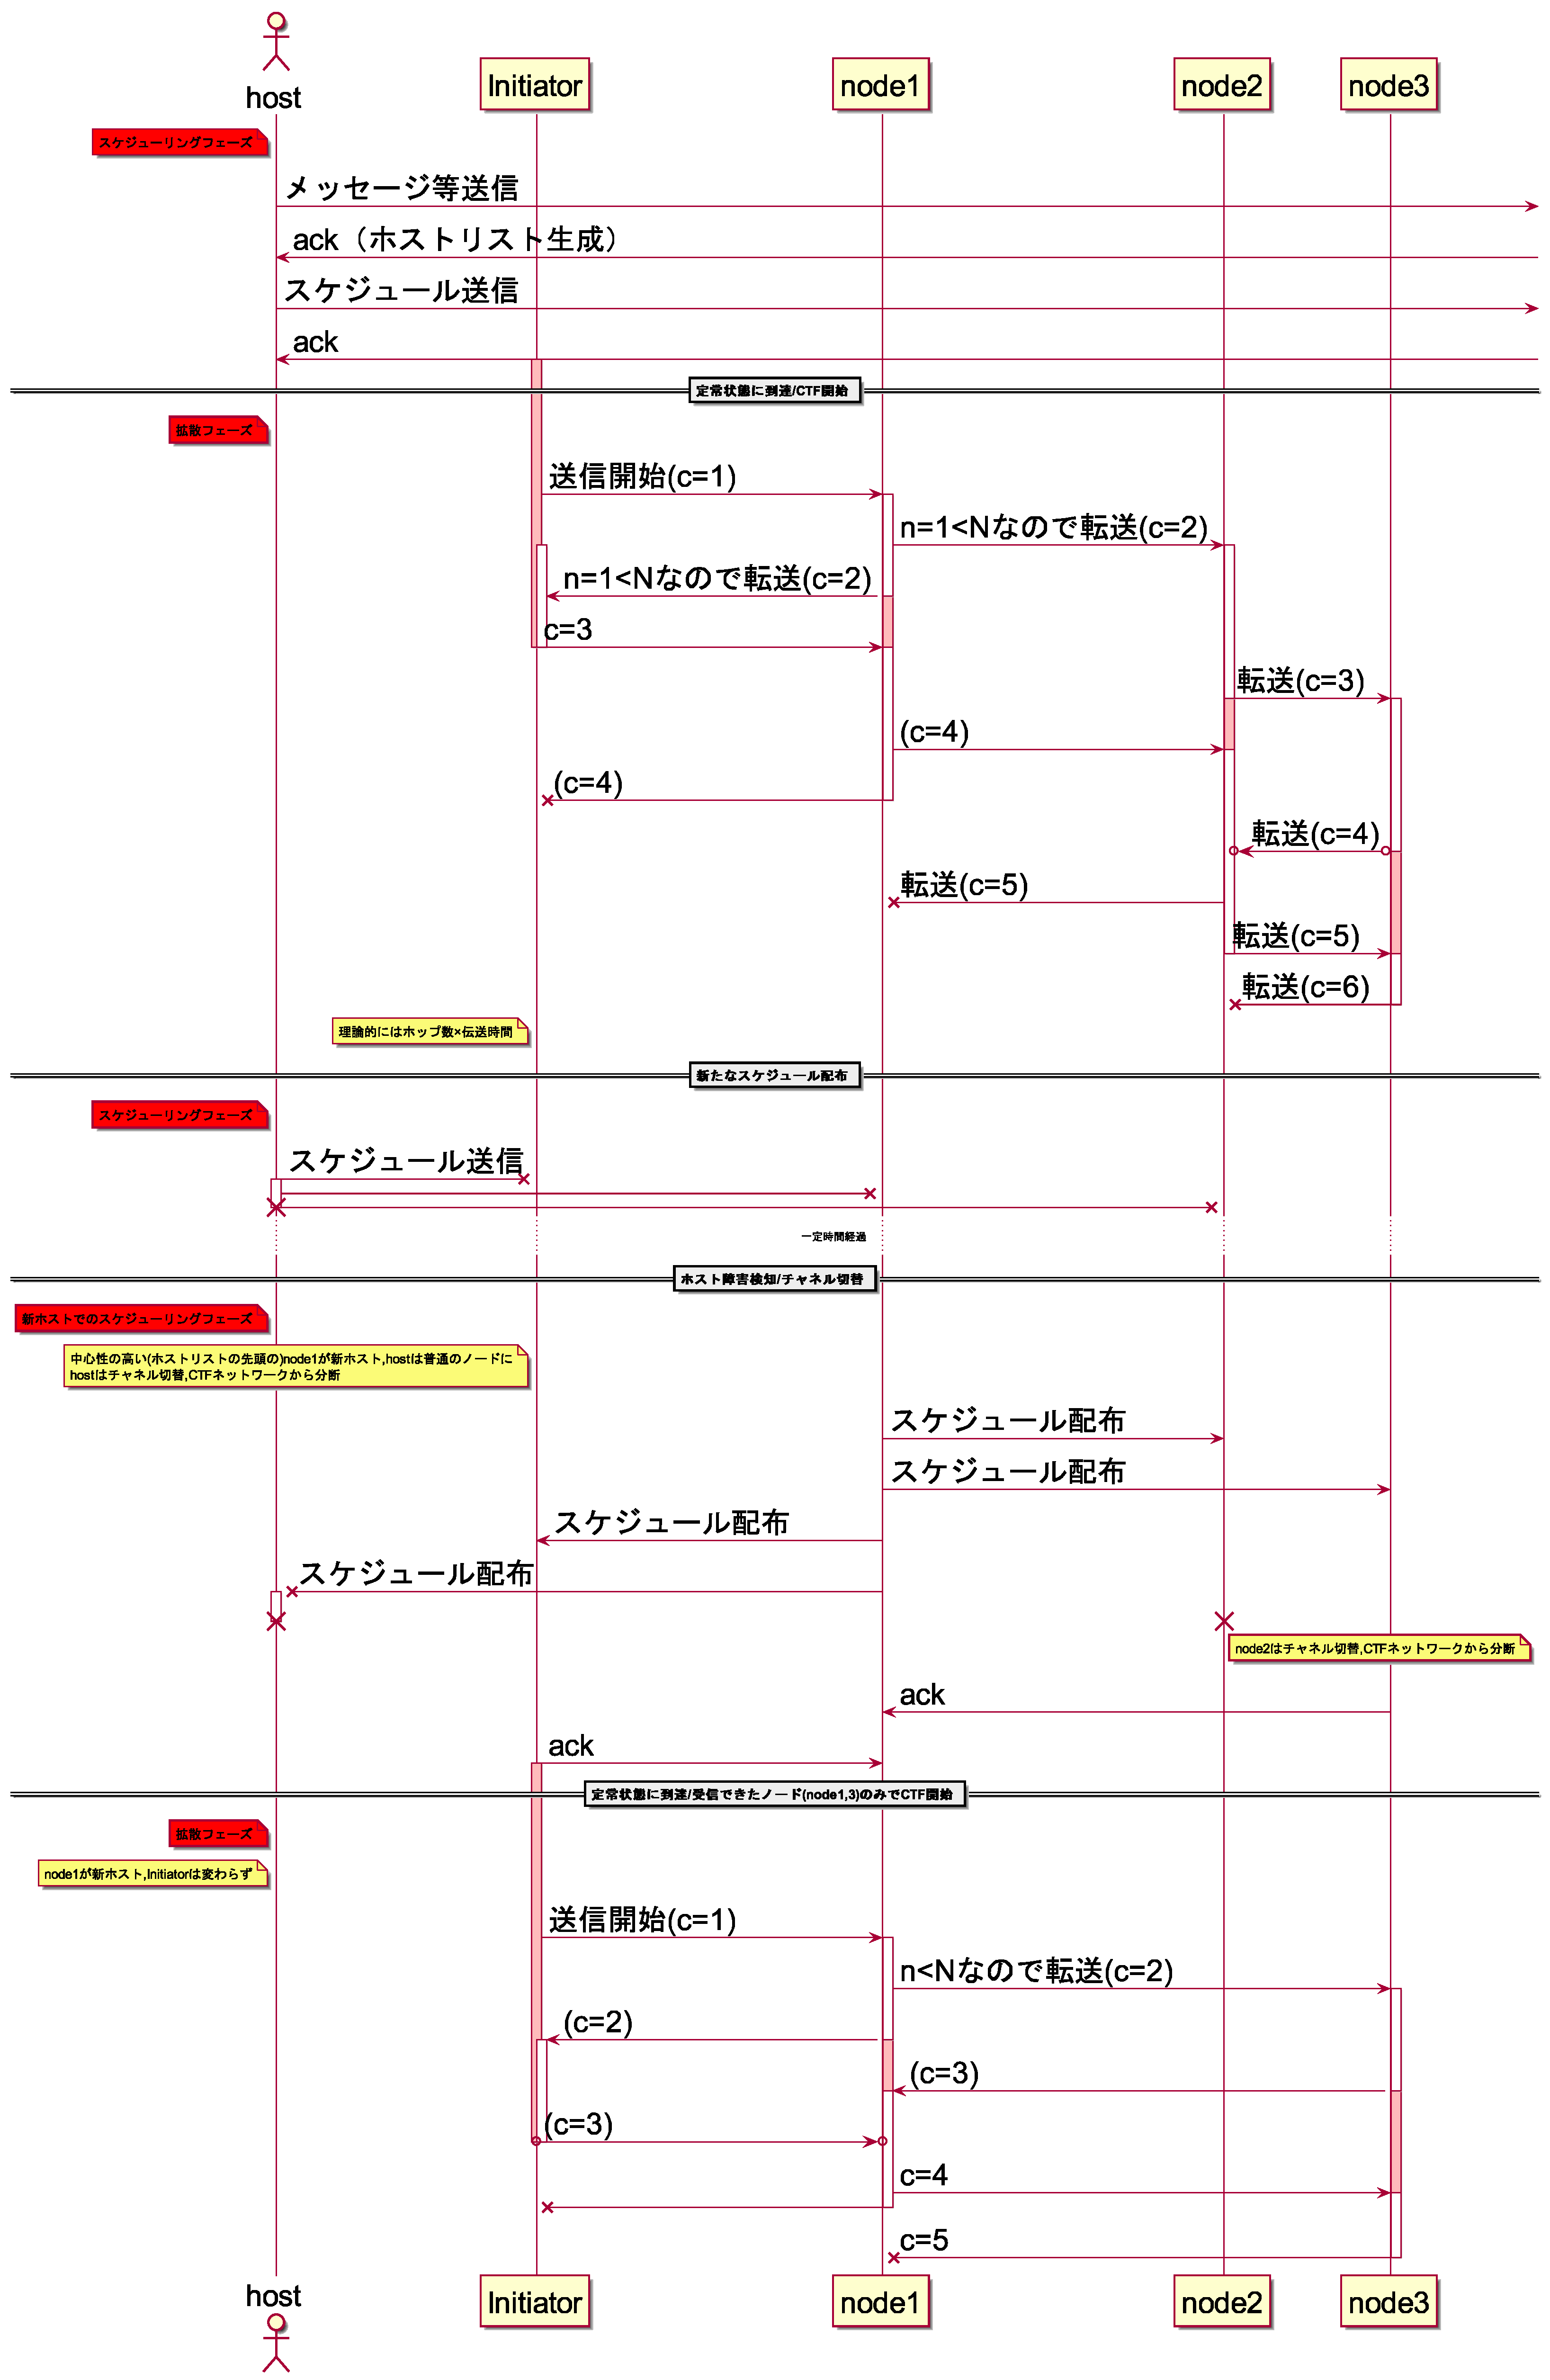
\includegraphics[width=1\textwidth]{figures/sequence_teian.eps}
  \caption{同時送信フラッディングの提案フローチャート}
  \label{fig:ctf_te}
\end{figure}

\section{ネットワークとグラフ}
\cite{network}によると,頂点と辺の具体的な関係性をネットワークという.本研究においてセンサを頂点,センサ同士の通信を辺と見なせばこれらの関係性もネットワークであると言える.またこれらは,頂点集合をV,辺の集合をEとすると,グラフG=(V,E)で定義できる.また,頂点間の繋がりが双方向なグラフを無向グラフという.本研究では無向グラフを考える.
また,どの頂点と頂点が繋がっているかを0と1で表す行列を隣接行列という.本研究で無向グラフを考えるため,隣接行列Aは対称であり,a[i,j]=a[j,i]となる.なおノードが自身から自身へ通信を行うことはあり得ないため,隣接行列の対角成分は0とする.図\ref{fig:adj}に示す.

\begin{figure}[H]
  \centering
  \includegraphics[width=0.8\textwidth]{figures/9.pdf}
  \caption{ノードと隣接行列}
  \label{fig:adj}
\end{figure}

\section{ホスト選択指標}
ホスト適性は,ノードの中心性に基づき評価を行う.
一般に,中心性とはネットワーク上におけるノードの重要性を評価するための指標であり,主な中心性の指標として媒介中心性や次数中心性が知られている.
\subsection*{媒介中心性}
媒介中心性は,そのノードが最短経路にどれくらい含まれるかを示す値である.この値が高いノードは,そのノードが失われたときにネットワーク全体に重大な影響を及ぼすことを意味する.本研究では,ネットワーク分断を避けるため,媒介中心性の高いノードをホストノードとしたい.そのためホスト選択指標として媒介中心性を使用する.あるグラフの隣接行列G=($g_{jk}$)を考えるとき,媒介中心性は以下の式\ref{eq_bet}で表せる.なお,$C_{b}(i)$は頂点iの媒介中心性,nはグラフ内の頂点数である.$g_{jk}$は頂点jと頂点kの間の全最短経路数で,$g_{jk}(i)$はその中で頂点iを通る数である.
\begin{equation}
\label{eq_bet}
C_{b}(i)=\sum_{i\neq j\neq l} \frac{g_{jk}(i)}{g_{jk}}
\end{equation}
\subsection*{次数中心性}
次数は,頂点に接続している辺の数である.次数中心性とはより多くの頂点と繋がっている頂点を高く評価する指標である.
本研究では,できるだけ多くのノードと通信可能なノードをホストノードとしたい.そのためホスト選択に次数中心性を使用する.あるグラフの隣接行列G=($g_{ij}$)を考えるとき,次数中心性は以下の式\ref{eq_deg}で表せる.なお,$C_{d}(i)$は頂点iの次数中心性,nはグラフ内の頂点数である.
\begin{equation}
\label{eq_deg}
C_{d}(i)=\sum_{j=1}^{n} a_{ij}=\sum_{j=1}^{n} a_{ji}
\end{equation}

\section{評価指標}
評価指標にはホストノードから全てのホストノード以外のノードへの最短経路長の平均と,Infの数を使う.ダイクストラ法で生成された最短経路行列d[i,j]において,ノードiとノードjの間に最短経路がないと判定されたとき,d[i,j]=Infとなる.この個数をInf数とする.
最短経路長平均が短ければ,理論上はホップ数$\times$伝送時間でネットワーク全体へのデータ転送が可能な同時送信フラッディングにおいての性能向上につながると考えた.また,Inf数が少なければ,ネットワーク全体の連結度が高いということであり,ネットワーク分断が起きづらくなるのではと考えた.なお,最短経路長はダイクストラ法によって求める.また,ノード数が異なる場合でも比較を行えるよう,Inf数の評価はInf数/全経路数の割合[\%]で評価を行う.

\subsection*{ダイクストラ法}
ダイクストラ法とはあるノードからあるノードまでの最短経路長を求めるアルゴリズムである.計算量はO(V\^2)である.無向グラフでかつ重みが負でない時に使える.ここで重みとは辺のコストを意味する.今回は重みは全て1とする.以下にダイクストラ法の手順を示す.なお.$d_{j}$は始点から頂点jまでの経路長,l[i,j]は頂点iと頂点jの間につながりがあるかどうか(あれば1,なければ0)を表す.

\begin{itemize}
    \item 行列L(対角成分が0,連結しているノード同士は1,それ以外は∞)を作成
    \item 始点から各頂点への距離行列dを作成(最初は始点が0,始点以外は∞)
    \item 距離が未確定な頂点のリストである行列Mを作る(最初は始点以外の全ての頂点をもつ)
    \item Mが空行列になるまで以下の3手順を繰り返す
    \item $d_j> d_i + l_{ij} ならば d_j = d_i + l_{ij}$
    \item 頂点iからの距離が最小な頂点kをMから消す  $\underset{j\in M}{\min} d_j=d_k$
    \item i=kでiを更新
\end{itemize}

疑似コードは以下の通りである.

\begin{algorithm}                    
\caption{dijkstra}         
\label{alg1}                          
\begin{algorithmic}[1] 
%REQUIREはInput,ENSUREはOutput
\REQUIRE 隣接行列matrix  始点vertex
\ENSURE 距離行列d
\WHILE{$Length(M) > 0$}
\FOR{j=1 to n}
\IF{$f[j]$ is finite}
\STATE $allf \Leftarrow $c(allf,f[j])
\ELSE
\STATE $num_inf \Leftarrow num_inf+1$
\ENDIF
\ENDFOR
    \STATE $i \Leftarrow M[which(f[M] = min(f[M]))[1]]$
	\STATE $M \Leftarrow M[-which(M=i)]$
\ENDWHILE
\end{algorithmic}
\end{algorithm}

行列Mは距離が未確定な頂点のリストである.つまり,最初の段階ではMは始点以外の全ての頂点を保持している.Mが空行列になるまで後述の処理を繰り返す[1行目].

また,上記で算出した最短経路長の中には,Infと対角成分の0が含まれるため,それらを除外する処理を行ったのち,最短経路長平均を求めた.

\chapter{シミュレーションの結果と考察}
%数値の取り直し,プロットエリアの見直しと枠をつける
%考察書く

本章では,前章で述べた同時送信フラッディングにおけるホスト選択手法をシミュレーションによって評価した結果について述べる.

\section{シミュレーション諸元}
媒介中心性と次数中心性はRのパッケージigraph内の関数betweennessと関数degreeで求めた.次数中心性と媒介中心性,それぞれの上位10\%ノードをホストノードにした場合とランダムに選んだ10\%ノードをホストノードに選んだときの比較を行う.
シミュレーションには,統計解析向けのプログラム言語であるR~\cite{R}を用いた.Rは機械学習やネットワーク分析のパッケージも豊富である.本研究では主にRのパッケージの一つであるigraphを使用した.
デフォルトではコアを1つしか使わない設定で,シミュレーションに時間がかかってしまうため,parallelパッケージとSNOWパッケージを使用し,並列化することでシミュレーション時間の短縮を図った.使用したRのバージョンやパッケージを表\ref{tab:sim_info}に示す.

\begin{table}[H]
\centering
  \caption{シミュレーション環境}
  \begin{tabular}{c|c} \hline\hline
    項目 & 内容  \\ \hline 
    package& parallel doSNOW  xlsx dplyr igraph\\
    R & R x64 3.6.1\\\hline\hline
  \end{tabular}
  \label{tab:sim_info}
\end{table}
%パッケージ説明
doSNOWパッケージとparallelパッケージは並列化に用いた.

シミュレーションに用いたパラメータは表\ref{tab:para_info}である.
\begin{table}[H]
\centering
  \caption{シミュレーション環境}
  \begin{tabular}{c|c|c} \hline\hline 
    項目 & 変数& 値  \\ \hline 
    ノード数& N & 50,100\\
    位置範囲& range & 250\\
    ホストノード数& host & 5,10\\
    到達範囲 & reach &20,30,40,50\\\hline\hline
  \end{tabular}
  \label{tab:para_info}
\end{table}

まず,250を上限としてランダムに生成した乱数を行列d(N,2)に代入し,ノードのxy座標とした.図\ref{fig:plotnode}は,これをプロットした一例である.x軸のd[,1]は行列dの1行目,y軸のd[,2]は行列dの2行目を表しており,これがx座標とy座標に対応している.単位は\si{\meter}である.


\begin{figure}[H]
  \centering
  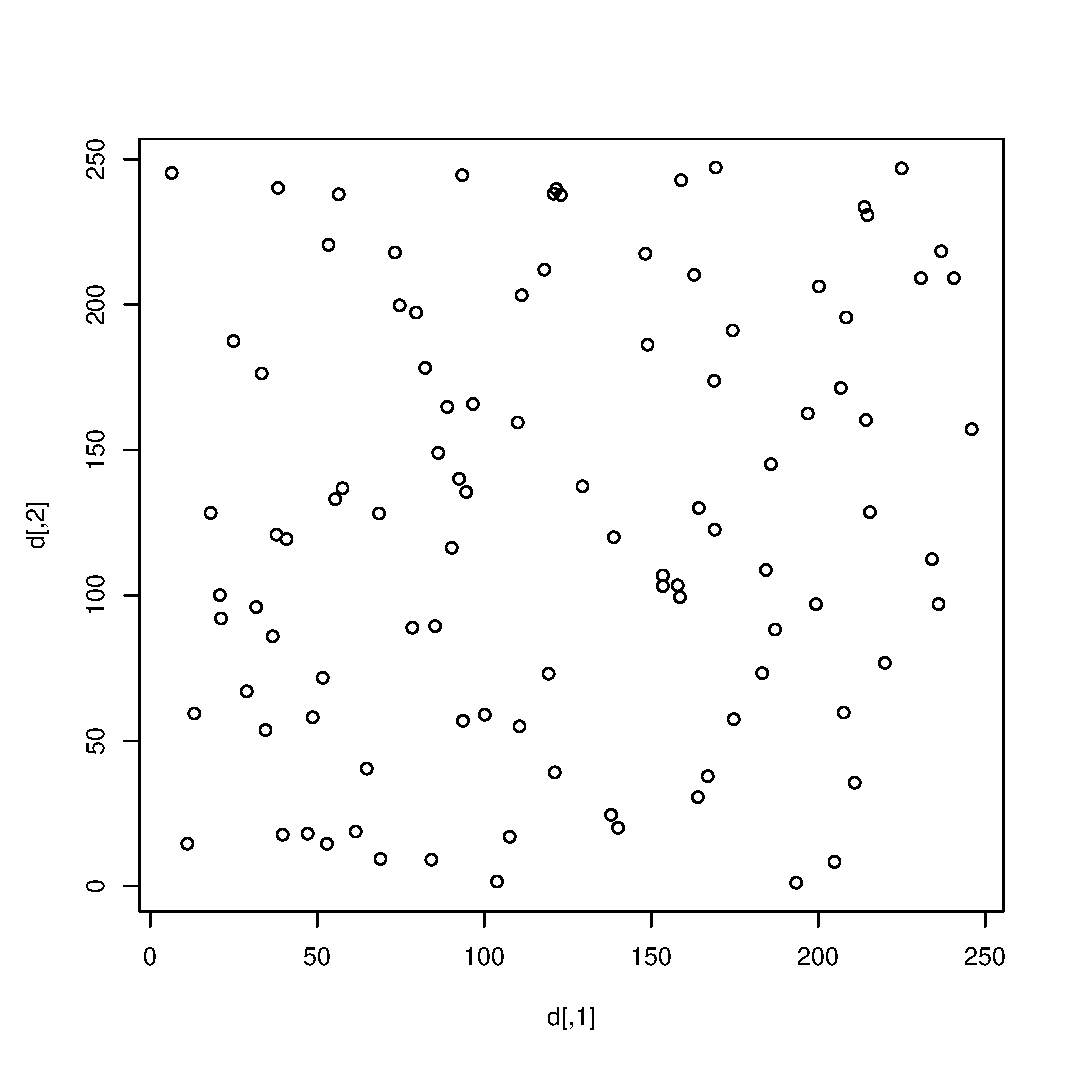
\includegraphics[width=0.8\textwidth]{figures/plotnode.eps}
  \caption{ノード位置}
  \label{fig:plotnode}
\end{figure}

その後,方法1は距離をしきい値としてその範囲内であれば完全に到達するという状況で,方法2は距離に反比例して下がる到達確率によって到達判定を行い,ネットワークグラフを作成した.生成されたネットワークグラフの一例を図\ref{fig:plotgraph}に示す.
\begin{figure}[H]
  \centering
  \includegraphics[width=0.8\textwidth]{figures/plotg.png}
  \caption{図\ref{fig:plotnode}から生成したネットワークグラフ}
  \label{fig:plotgraph}
\end{figure}

それぞれにおいて媒介中心性と次数中心性の上位10\%ノードをホストノードとした際の最短経路長平均とInf数をダイクストラ法によって求めた.比較対象は,全ノードの10\%のノードをランダムに選出した際の最短経路長平均とInf数である.
また,ノードの配置による影響を除外するため,方法1,2ともに上記の過程をシード値を変更して1万回行った.

%%%%%%%%%%%%%%%%%%%%%%%%%方法1開始%%%%%%%%%%%%%%%%%%%%%%%%%%%%%%%%%%

\section{方法1:距離による到達判定}
方法1は到達距離を設定し,その範囲内であれば通信が100\%可能であるという状況を想定したシミュレーションである.媒介中心性と次数中心性で上位10\%ノードをホストノードとした時の最短経路長平均を表\ref{tab:1_spl_bet}に示す.なお,50ノードで到達範囲を20とした際,従来手法では,NAという値が含まれてしまい,最短経路長平均が求まらなかった.ノード密度が低いことと,到達範囲が狭いことで,通信が成立しなかったためと思われる.表にはNAを除外した値を載せている.そのためグラフ上は20\si{\meter}において平均最短経路長が短く出ているが,実際は最短経路長平均が存在しない(すべてのノードがつながっていない)状態を含んでいる.

\begin{comment}
\begin{table}[H]
\centering
\caption{方法1の平均最短経路長}
\scalebox{0.55}[0.55]{
  \begin{tabular}{c|c|c|c|c|c|c} \hline\hline
     到達距離 [\si{\meter}] & 50従来 [ホップ] &50媒介 [ホップ]&50次数 [ホップ] &100従来 [ホップ]& 100媒介 [ホップ]& 100次数 [ホップ]\\ \hline 
    20 & 1.343 & 1.346 & 1.277& 2.275 & 2.420 & 1.993\\
    30 & 2.161 & 2.123 & 1.858 & 5.295 & 4.487 & 4.497\\
    40 & 3.386 & 2.903 & 2.778 & 4.243 & 3.523 & 3.572\\
    50 & 3.451 & 2.824 & 2.780 & 3.196 & 2.691 & 2.697\\ \hline\hline
  \end{tabular}
  }
\label{tab:1_spl_bet}
\end{table}
\end{comment}

\begin{table}[H]
\centering
\caption{方法1の平均最短経路長}
\scalebox{1}[1]{
  \begin{tabular}{c|c|c|c|c} \hline\hline
 & 20 [\si{\meter}] & 30 [\si{\meter}] & 40 [\si{\meter}] &50 [\si{\meter}]\\ \hline
50従来 & 1.343 & 2.161 & 3.386 & 3.451 \\
50媒介 & 1.346 & 2.123 & 2.903 & 2.824 \\
50次数 & 1.277 & 1.858 & 2.778 & 2.78 \\ 
100従来 & 2.275 & 5.295 & 4.243 & 3.196 \\ 
100媒介 & 2.42 & 4.487 & 3.523 & 2.691 \\ 
100次数 & 1.993 & 4.497 & 3.572 & 2.697 \\ \hline\hline
  \end{tabular}
  }
\label{tab:1_spl_bet}
\end{table}

表\ref{tab:1_spl_bet}の内容を手法ごとにプロットしたものを図\ref{fig:1hopall}に示す.

\begin{figure}[H]
  \centering
  \includegraphics[width=1.05\textwidth]{figures/1spl.pdf}
  \caption{到達距離ごとの方法1の最短経路長平均}
  \label{fig:1hopall}
\end{figure}

いずれの場合においてもランダムに選んだ10\%ノードをホストノードとした従来手法よりもホスト選択を行った方が最短経路長平均が短い.また,媒介中心性でホスト選択したときと次数中心性でホスト選択したときを比較すると,ノード数に関わらず次数中心性の方がよい.しかし,到達距離が大きくなるにつれ2つの差は縮まり,ノードが50・100いずれの場合でも到達距離が50\si{\meter}のときはあまり差が見られない.

ここで50ノードと100ノードにおける次数中心性と媒介中心性の分布を図\ref{fig:50100bg}に示す.上2つのヒストグラムが50ノード,下2つが100ノードで,左側の2つのヒストグラムが媒介中心性の分布,右2つが次数中心性の分布を示している.

\begin{figure}[H]
  \centering
  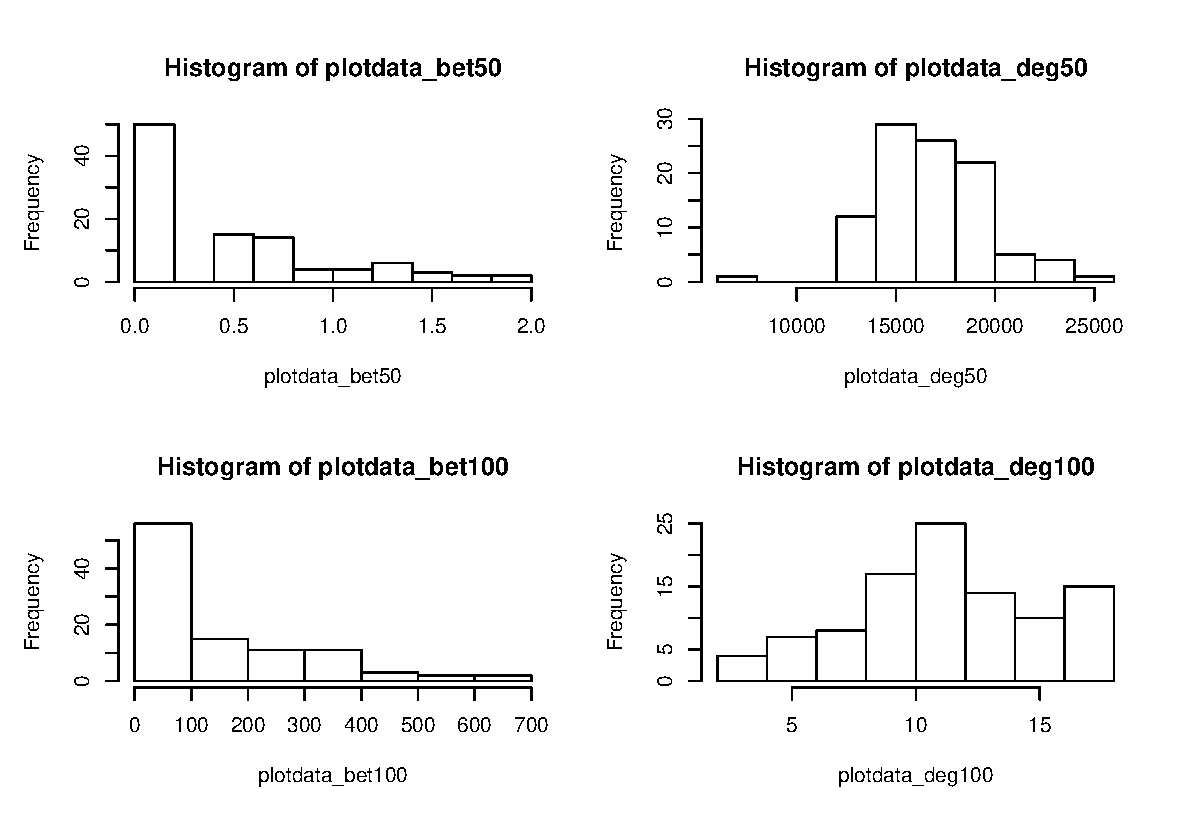
\includegraphics[width=1\textwidth]{figures/50100bg.eps}
  \caption{ノード数による媒介中心性と次数中心性の分布の違い}
  \label{fig:50100bg}
\end{figure}

ノード数によって次数中心性と媒介中心性の値の桁が大きく変わることがわかる.ノードの密度が高い50ノードにおいては,次数中心性が大きくなるのは自明であり,次数中心性がノードの密度に大きく影響されることがわかる.また,到達範囲が広がるということは通信可能範囲内のノードが増えるということでこれも間接的にノードの密度が大きくなっているといえる.
本研究では,次数中心性による選択の方が最短経路長平均が短くなったが,さらにノード数を増やし,ノード密度が大きくなる場合は,媒介中心性の方が最短経路長平均が短くなると推測される.
また,同時送信フラッディングの,ノード過密時は性能が下がるという特徴を考慮すると,ノードが密なときに性能がいい次数中心性によるホスト選択より媒介中心性によるホスト選択の方が同時送信フラッディングに適しているといえる.

%%%%%%%%%%%%%%%%%%%%%%↑方法1最短経路長平均%%%%%%%%%%%%%%%%%%%%%%%%%%

%%%%%%%%%%%%%%%%%%%%%%%%%%%↓方法1Inf数%%%%%%%%%%%%%%%%%%%%%%%%%%

\begin{comment}

\begin{table}[H]
\centering
  \caption{方法1のInf数}
\scalebox{0.55}[0.55]{
  \begin{tabular}{c|c|c|c|c|c|c} \hline\hline
    到達距離 [\si{\meter}] & 50従来 [個] &50媒介 [個]&50次数 [個] &100従来 [個]& 100媒介 [個]& 100次数 [個]\\ \hline 
    20 & 116,735,452(93.4\%) & 111,497,510(89.2\%) & 111,158,504(88.9\%) & 933,612,885(93.4\%) & 870,218,229(87.0\%) & 888,797,275(88.9\%)\\
    30 & 107,704,036(86.2\%) & 95,797,648(76.6\%)  & 98,417,647(78.7\%) & 641,037,650(64.1\%) & 536,432,013(53.6\%) & 578,549,885(57.9\%)\\
    40 & 81,753,752(65.4\%) & 67,507,031(54.0\%)   & 71,600,767(57.3\%) & 373,913,223 (37.4\%)& 339,721,118(34.0\%) & 362,988,951(36.3\%)\\
    50 & 52,258,853 (41.8\%)& 44,334,309(35.5\%)& 47,604,897(38.1\%) & 296,649,201(29.7\%) & 258,705,947(25.9\%) & 290,858,488(29.1\%)\\ \hline\hline
  \end{tabular}
  }
  \label{tab:1_inf}
\end{table}
\end{comment}

\begin{table}[H]
\centering
  \caption{方法1のInf数}
\scalebox{1}[1]{
  \begin{tabular}{c|c|c|c|c} \hline\hline
 &20 [\si{\meter}] & 30 [\si{\meter}] & 40 [\si{\meter}] & 50 [\si{\meter}] \\ \hline
50従来 & 93.4 & 86.2 & 65.4 & 42 \\ 
50媒介 & 89.2 & 76.7 & 54 & 35.5 \\ 
50次数 & 88.9 & 78.7 & 57.3 & 38.1 \\ 
100従来 & 93.4 & 64.1 & 37.4 & 29.7 \\ 
100媒介 & 87 & 53.6 & 34 & 25.9 \\ 
100次数 & 88.9 & 57.9 & 36.3 & 29.1 \\ \hline\hline
  \end{tabular}
  }
  \label{tab:1_inf}
\end{table}







\begin{figure}[H]
  \centering
  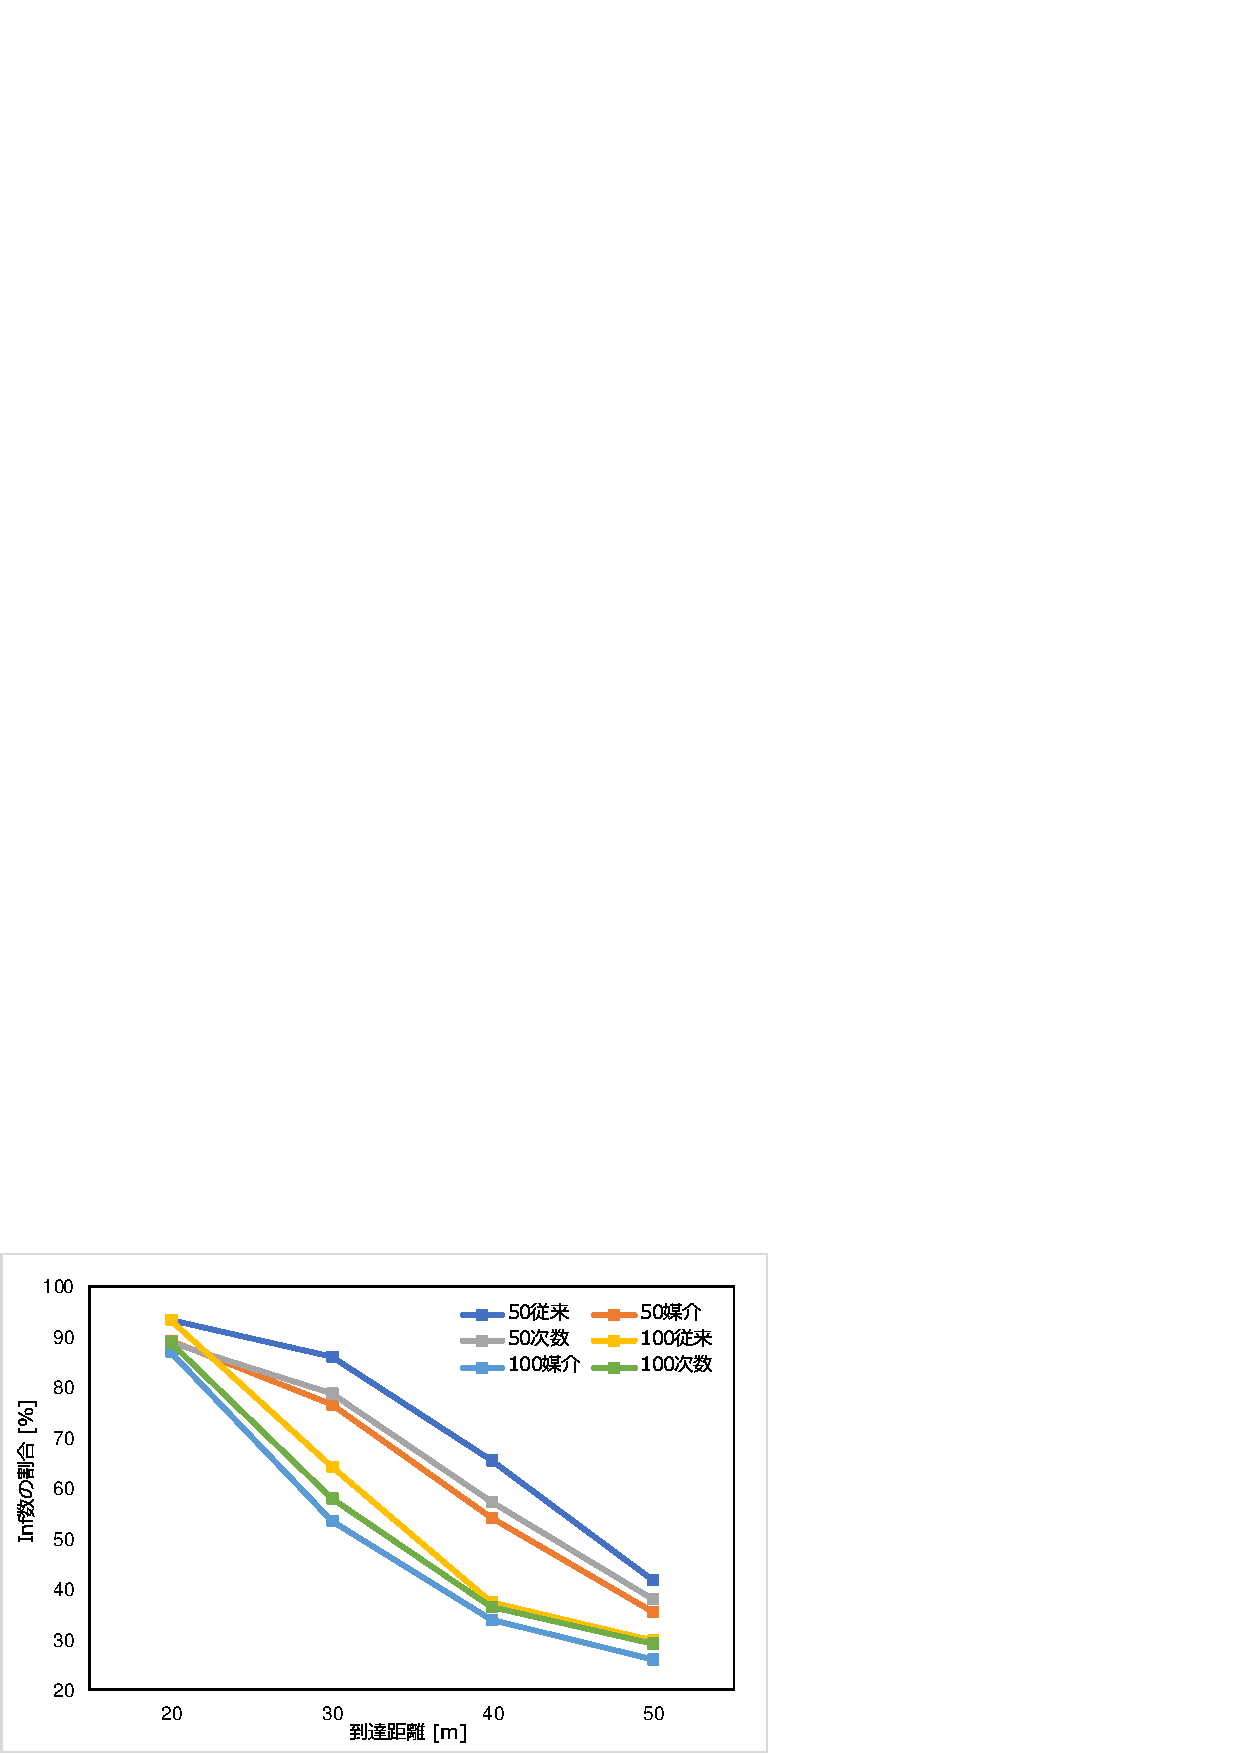
\includegraphics[width=1.05\textwidth]{figures/1Inf.pdf}
  \caption{到達距離ごとの方法1のInf数の割合}
  \label{fig:1Infall}
\end{figure}
方法1におけるInf数はノード数が50,到達範囲が20\si{\meter}のときのみ次数中心性がわずかによく,それ以外においては媒介中心性がよいことがわかった.先述のように50ノードで到達範囲が20\si{\meter}のときは例外的な値を含んでいるため,ここでは除外する.
また,到達距離に反比例してInf数の割合が下がることが見て取れるが,これはノード密度が大きくなるためだと考えられる.
また,100ノードで到達距離が50\si{\meter}のときは,従来手法と提案手法の差が小さいこともわかる.ノード密度が大きい場合は,ホストノードをランダムに選んだ場合でも,ネットワーク分断の可能性が小さくなることが示唆されている.一方,50ノードにおいては従来手法と提案手法の差は大きく,ノード密度が小さい状況においてはホストノードを中心性によって選出することの有効性が確認できた.
%%%%%%%%%%%%%%%%%%%%%%%%%方法2開始%%%%%%%%%%%%%%%%%%%%%%%%%%%%%%%%%%

\section{方法2:確率による到達判定}
次にノイズ等の影響により通信が失敗した状況を想定し,距離の2乗に反比例する確率による到達判定を行った.方法1では設定した到達距離内であれば100\%通信が可能であるとしてシミュレーションを行ったが,方法2においては近くても失敗する可能性があり,遠くても成功する可能性があるという状態でシミュレーションを行った.

\begin{table}[H]
    \centering
  \caption{方法2の平均最短経路長}
\scalebox{0.5}[0.5]{
  \begin{tabular}{c|c|c|c|c|c} \hline\hline
       50従来 [ホップ] &50提案(媒介) [ホップ]&50提案(次数) [ホップ] &100従来 [ホップ]& 100提案(媒介) [ホップ]& 100提案(次数) [ホップ] \\ \hline 
       2.086 & 1.792 & 1.740 & 2.001 & 1.756 & 1.733\\ \hline\hline
  \end{tabular}
  }
  \label{tab:2_spl}
\end{table}


\begin{figure}[H]
  \centering
  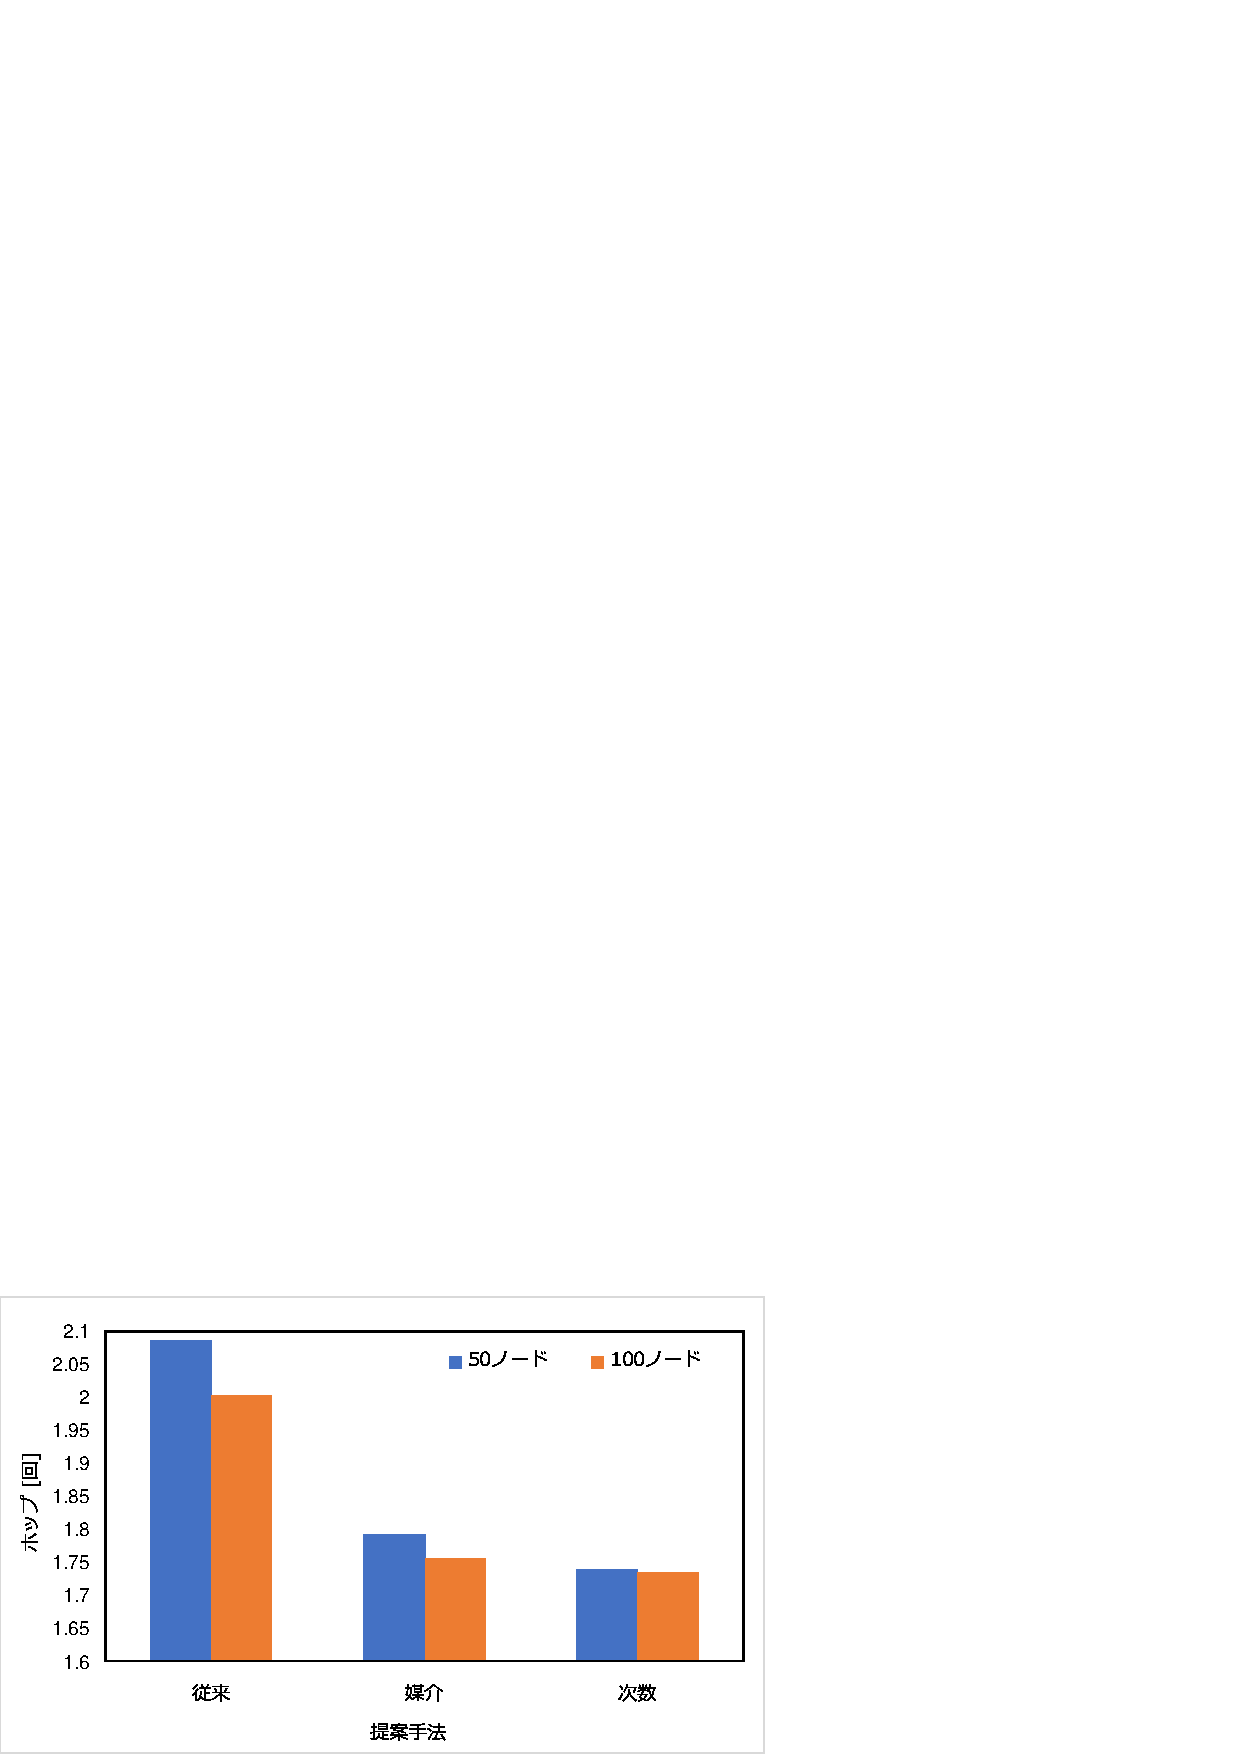
\includegraphics[width=1\textwidth]{figures/2hop.pdf}
    \vspace{-20mm}
  \caption{方法2の最短経路長平均}   
  \label{fig:2hop}
\end{figure}

いずれの提案手法も従来手法に比べて最短経路長平均が小さく,従来のリストによるラウンドロビン方式のホスト選択より,到達性を考慮してホスト選択を行った方がよいということがわかった.
また,媒介中心性でホスト選択した場合と,次数中心性でホスト選択した場合では,ノード数に関係なく次数中心性による選択の方がよい結果となった.


\begin{table}[H]
    \centering
  \caption{方法2のInf数}
\scalebox{0.55}[0.55]{
  \begin{tabular}{c|c|c|c|c|c|c} \hline\hline
       50従来 [個] &50媒介 [個]&50次数 [個] &100従来 [個]& 100媒介 [個]& 100次数 [個] \\ \hline 
      22,467,967(18.0\%) & 16,491,898(13.2\%) &19,554,978(15.6\%)& 130,496,056(13.0\%) & 83,183,195(8.32\%)& 100,239,883(10.0\%) \\ \hline\hline
  \end{tabular}
  }
  \label{tab:2_inf}
\end{table}

\begin{figure}[H]
  \centering
  \includegraphics[width=1\textwidth]{figures/2inf.pdf}
  \label{fig:2Inf}
      \vspace{-20mm}
    \caption{方法2のInf数の割合}
\end{figure}

一方,Infの割合においては,ノード数が50のときでも100のときでも媒介中心性によるホスト選択が最もよい結果となった.
また方法1,2ともに50ノードのInf数が多いのは,ノードの密度が小さいことで繋がっている辺が少なくなるからであり,直感的にも納得のいく結果となった.


%%%%%%%%%%%%%%%%%%%%%%%%%グラフ%%%%%%%%%%%%%%%%%%%%%%%%%%%%%%%%%%

\section{全結果}
本研究のシミュレーションにおける全結果の累積分布関数プロットとヒストグラムを図\ref{fig:1_50_30}から図\ref{fig:2_100}に示す.
\begin{landscape}
\begin{figure}[H]
  \centering
  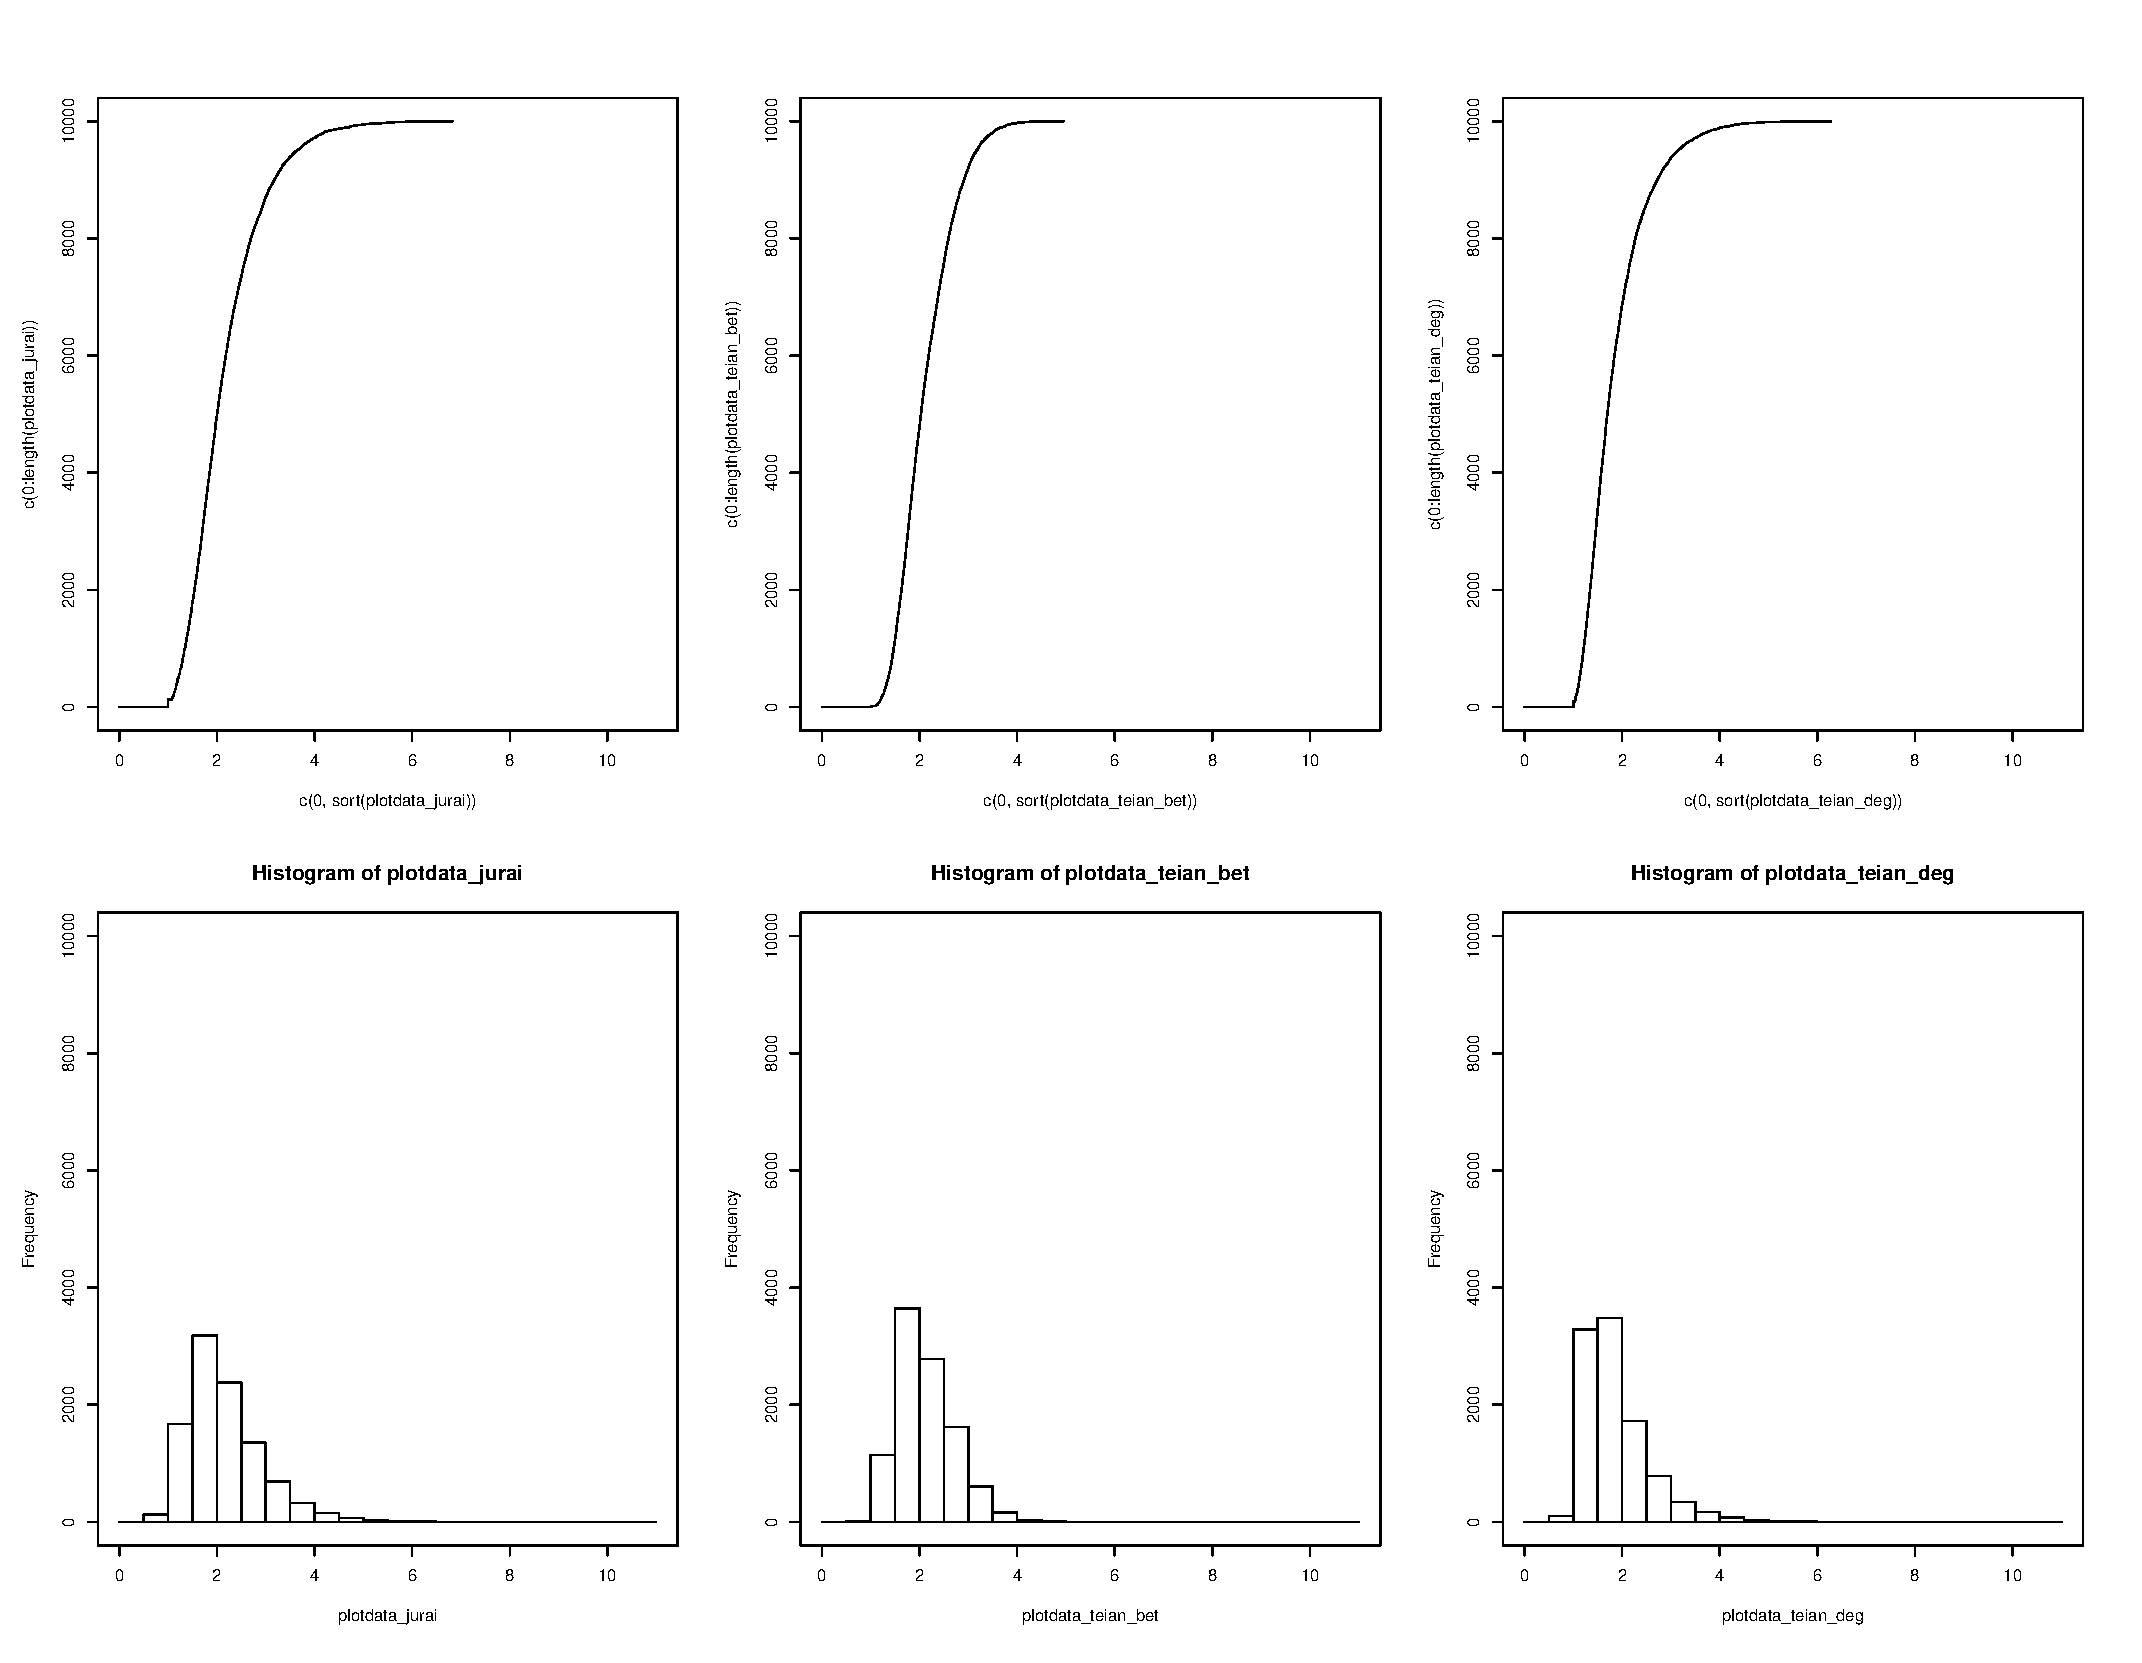
\includegraphics[width=1.2\textwidth]{figures/1_50_30.eps}
  \caption{方法1:50ノードで到達範囲を30としたとき}
  \label{fig:1_50_30}
\end{figure}

\begin{figure}[H]
  \centering
  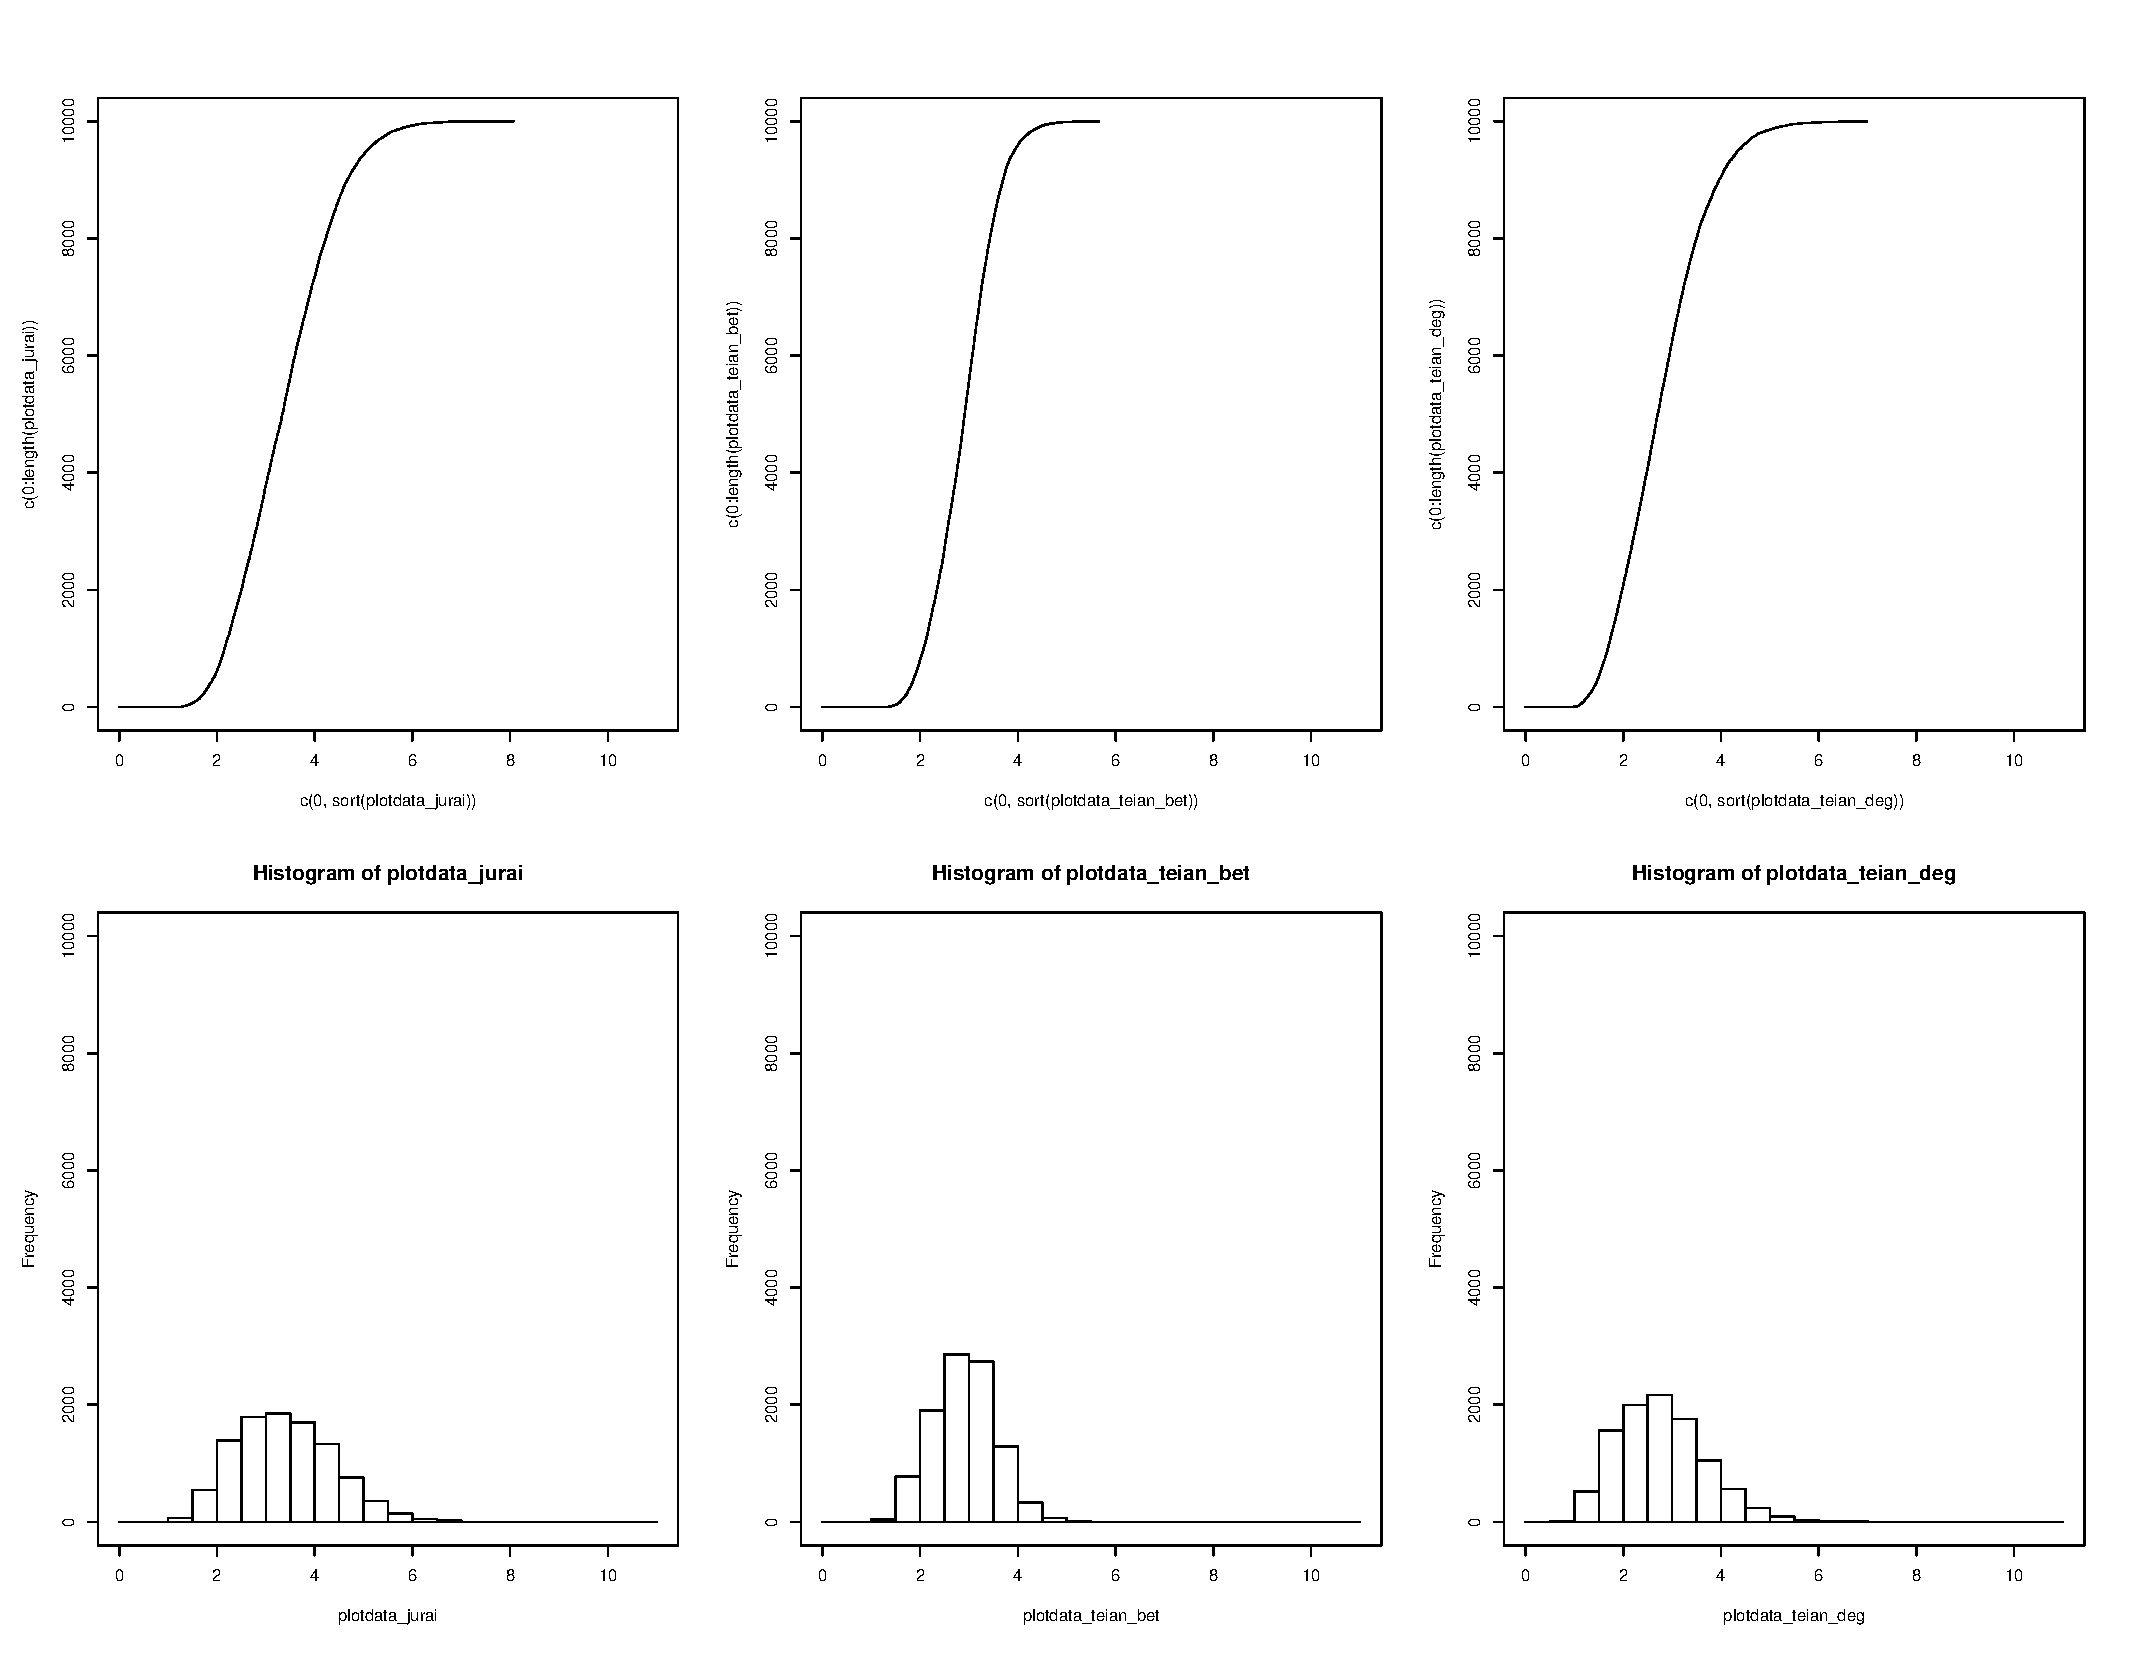
\includegraphics[width=1.2\textwidth]{figures/1_50_40.eps}
  \caption{方法1:50ノードで到達範囲を40としたとき}
  \label{fig:plot}
\end{figure}

\begin{figure}[H]
  \centering
  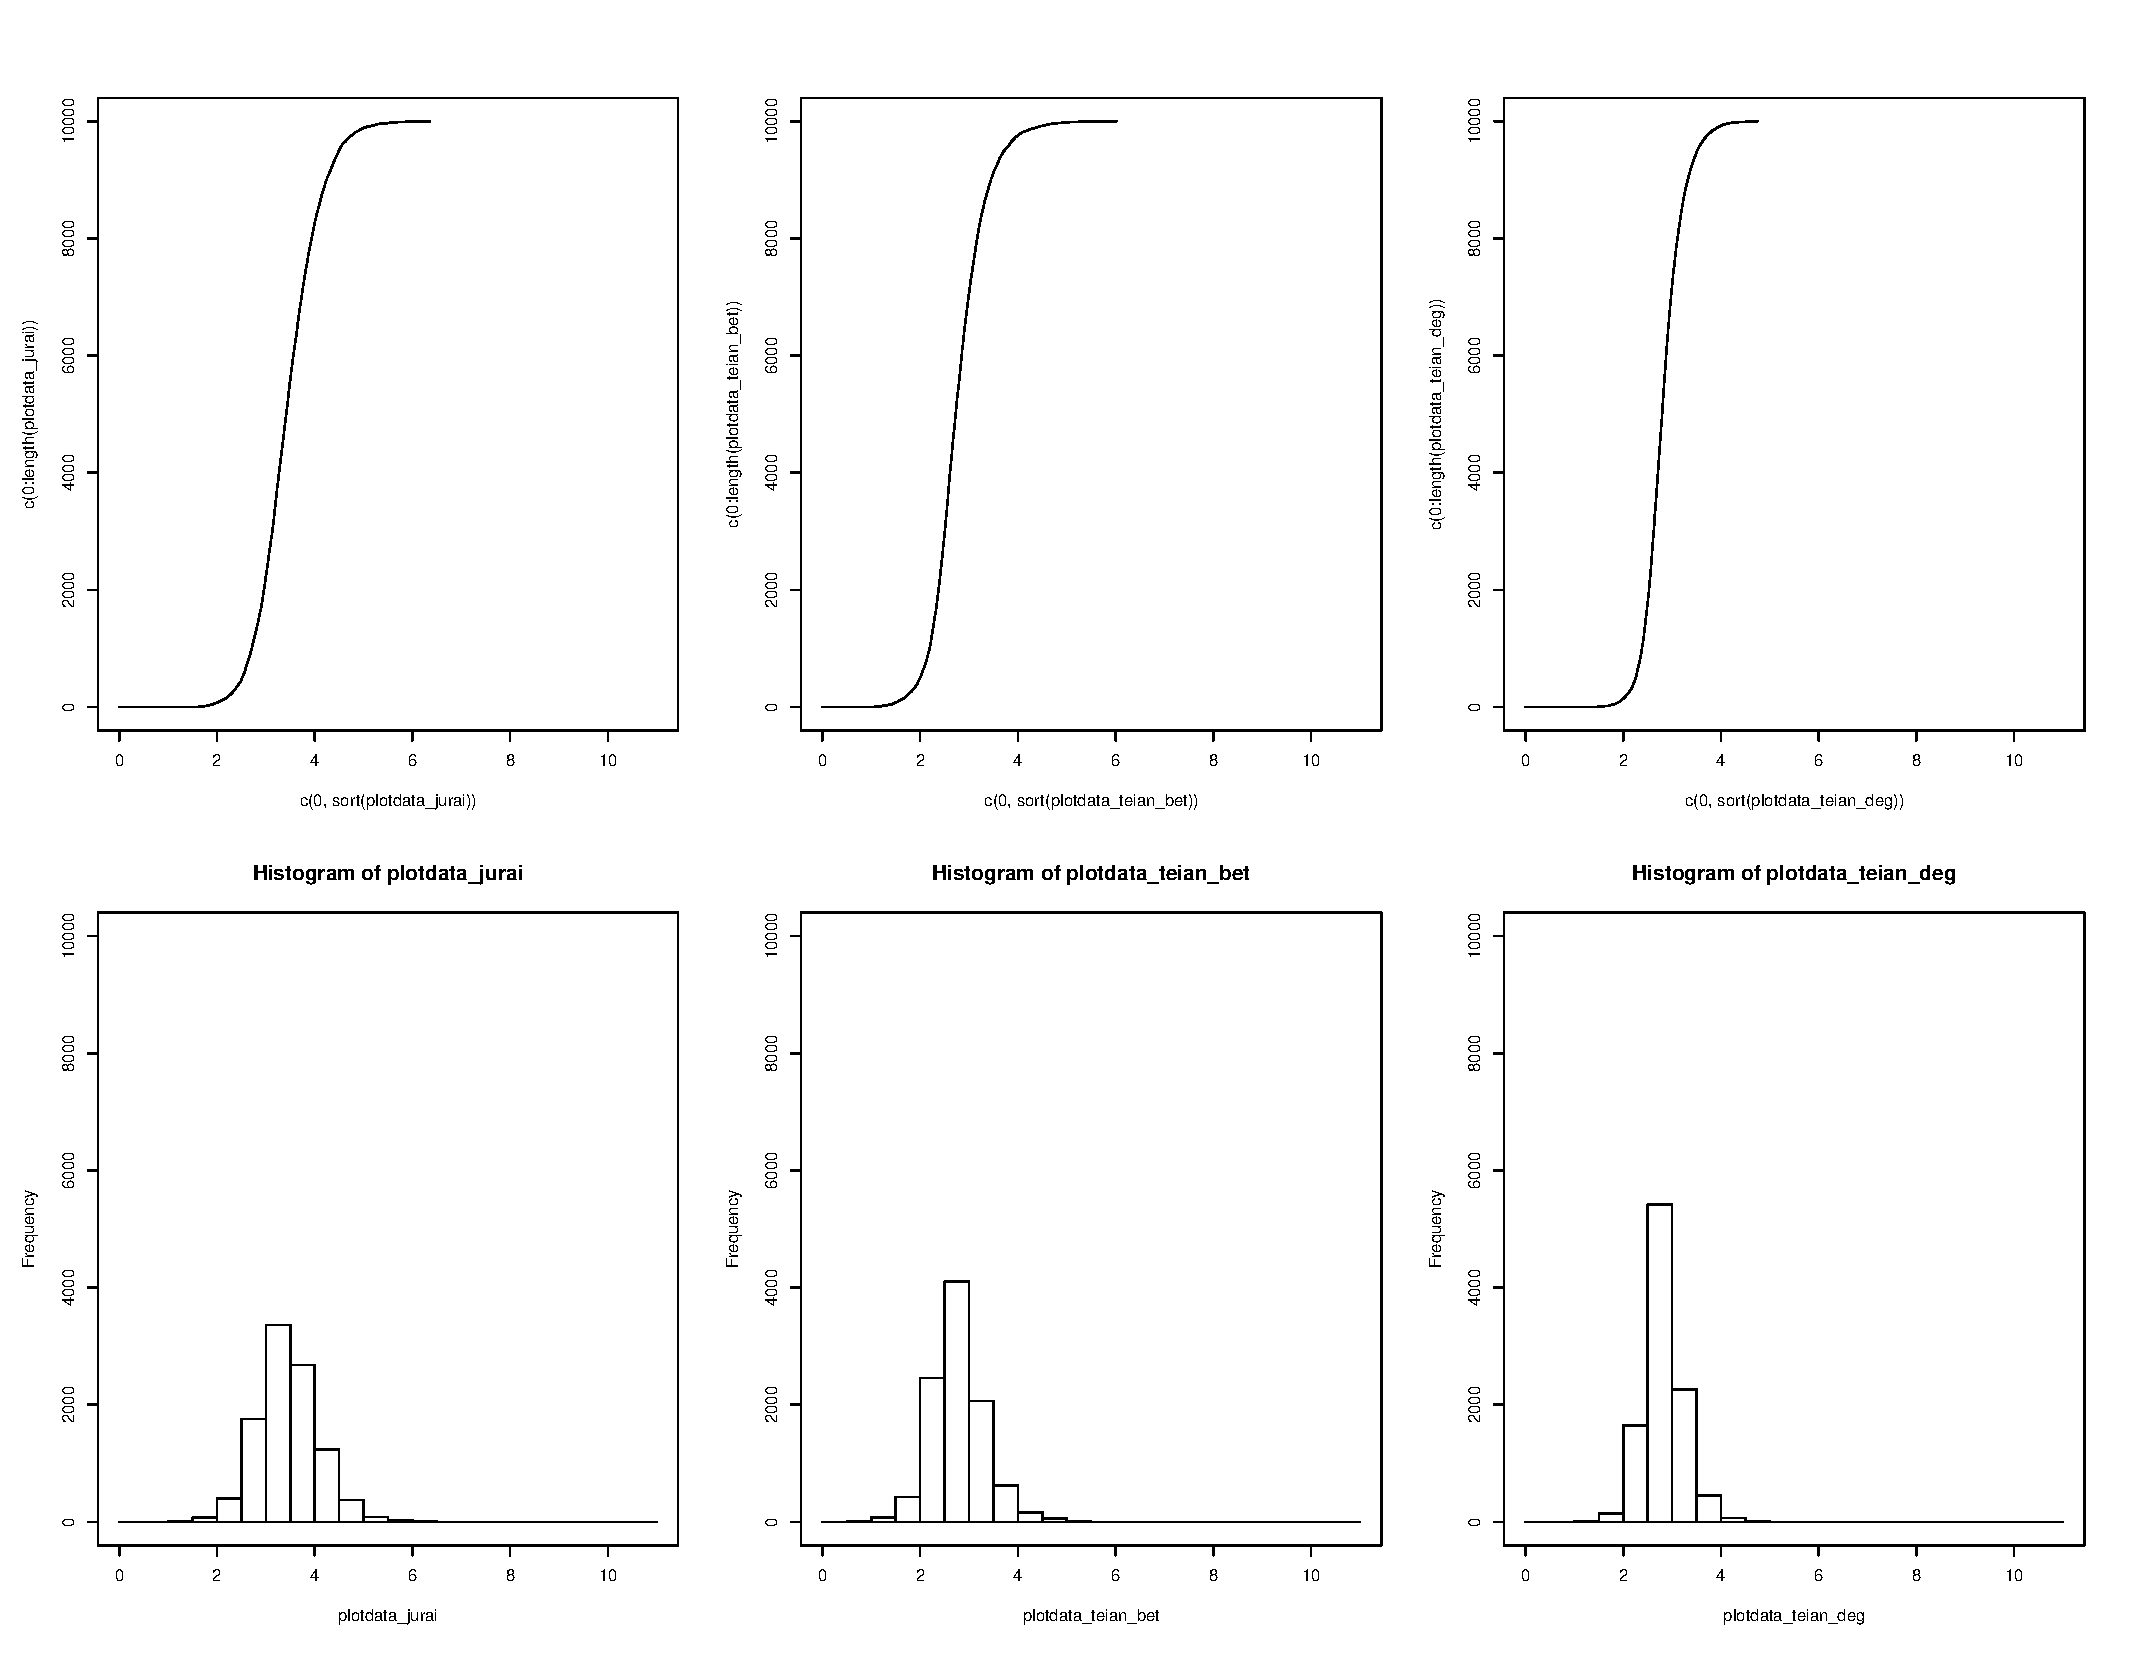
\includegraphics[width=1.2\textwidth]{figures/1_50_50.eps}
  \caption{方法1:50ノードで到達範囲を50としたとき}
  \label{fig:plot}
\end{figure}

\begin{figure}[H]
  \centering
  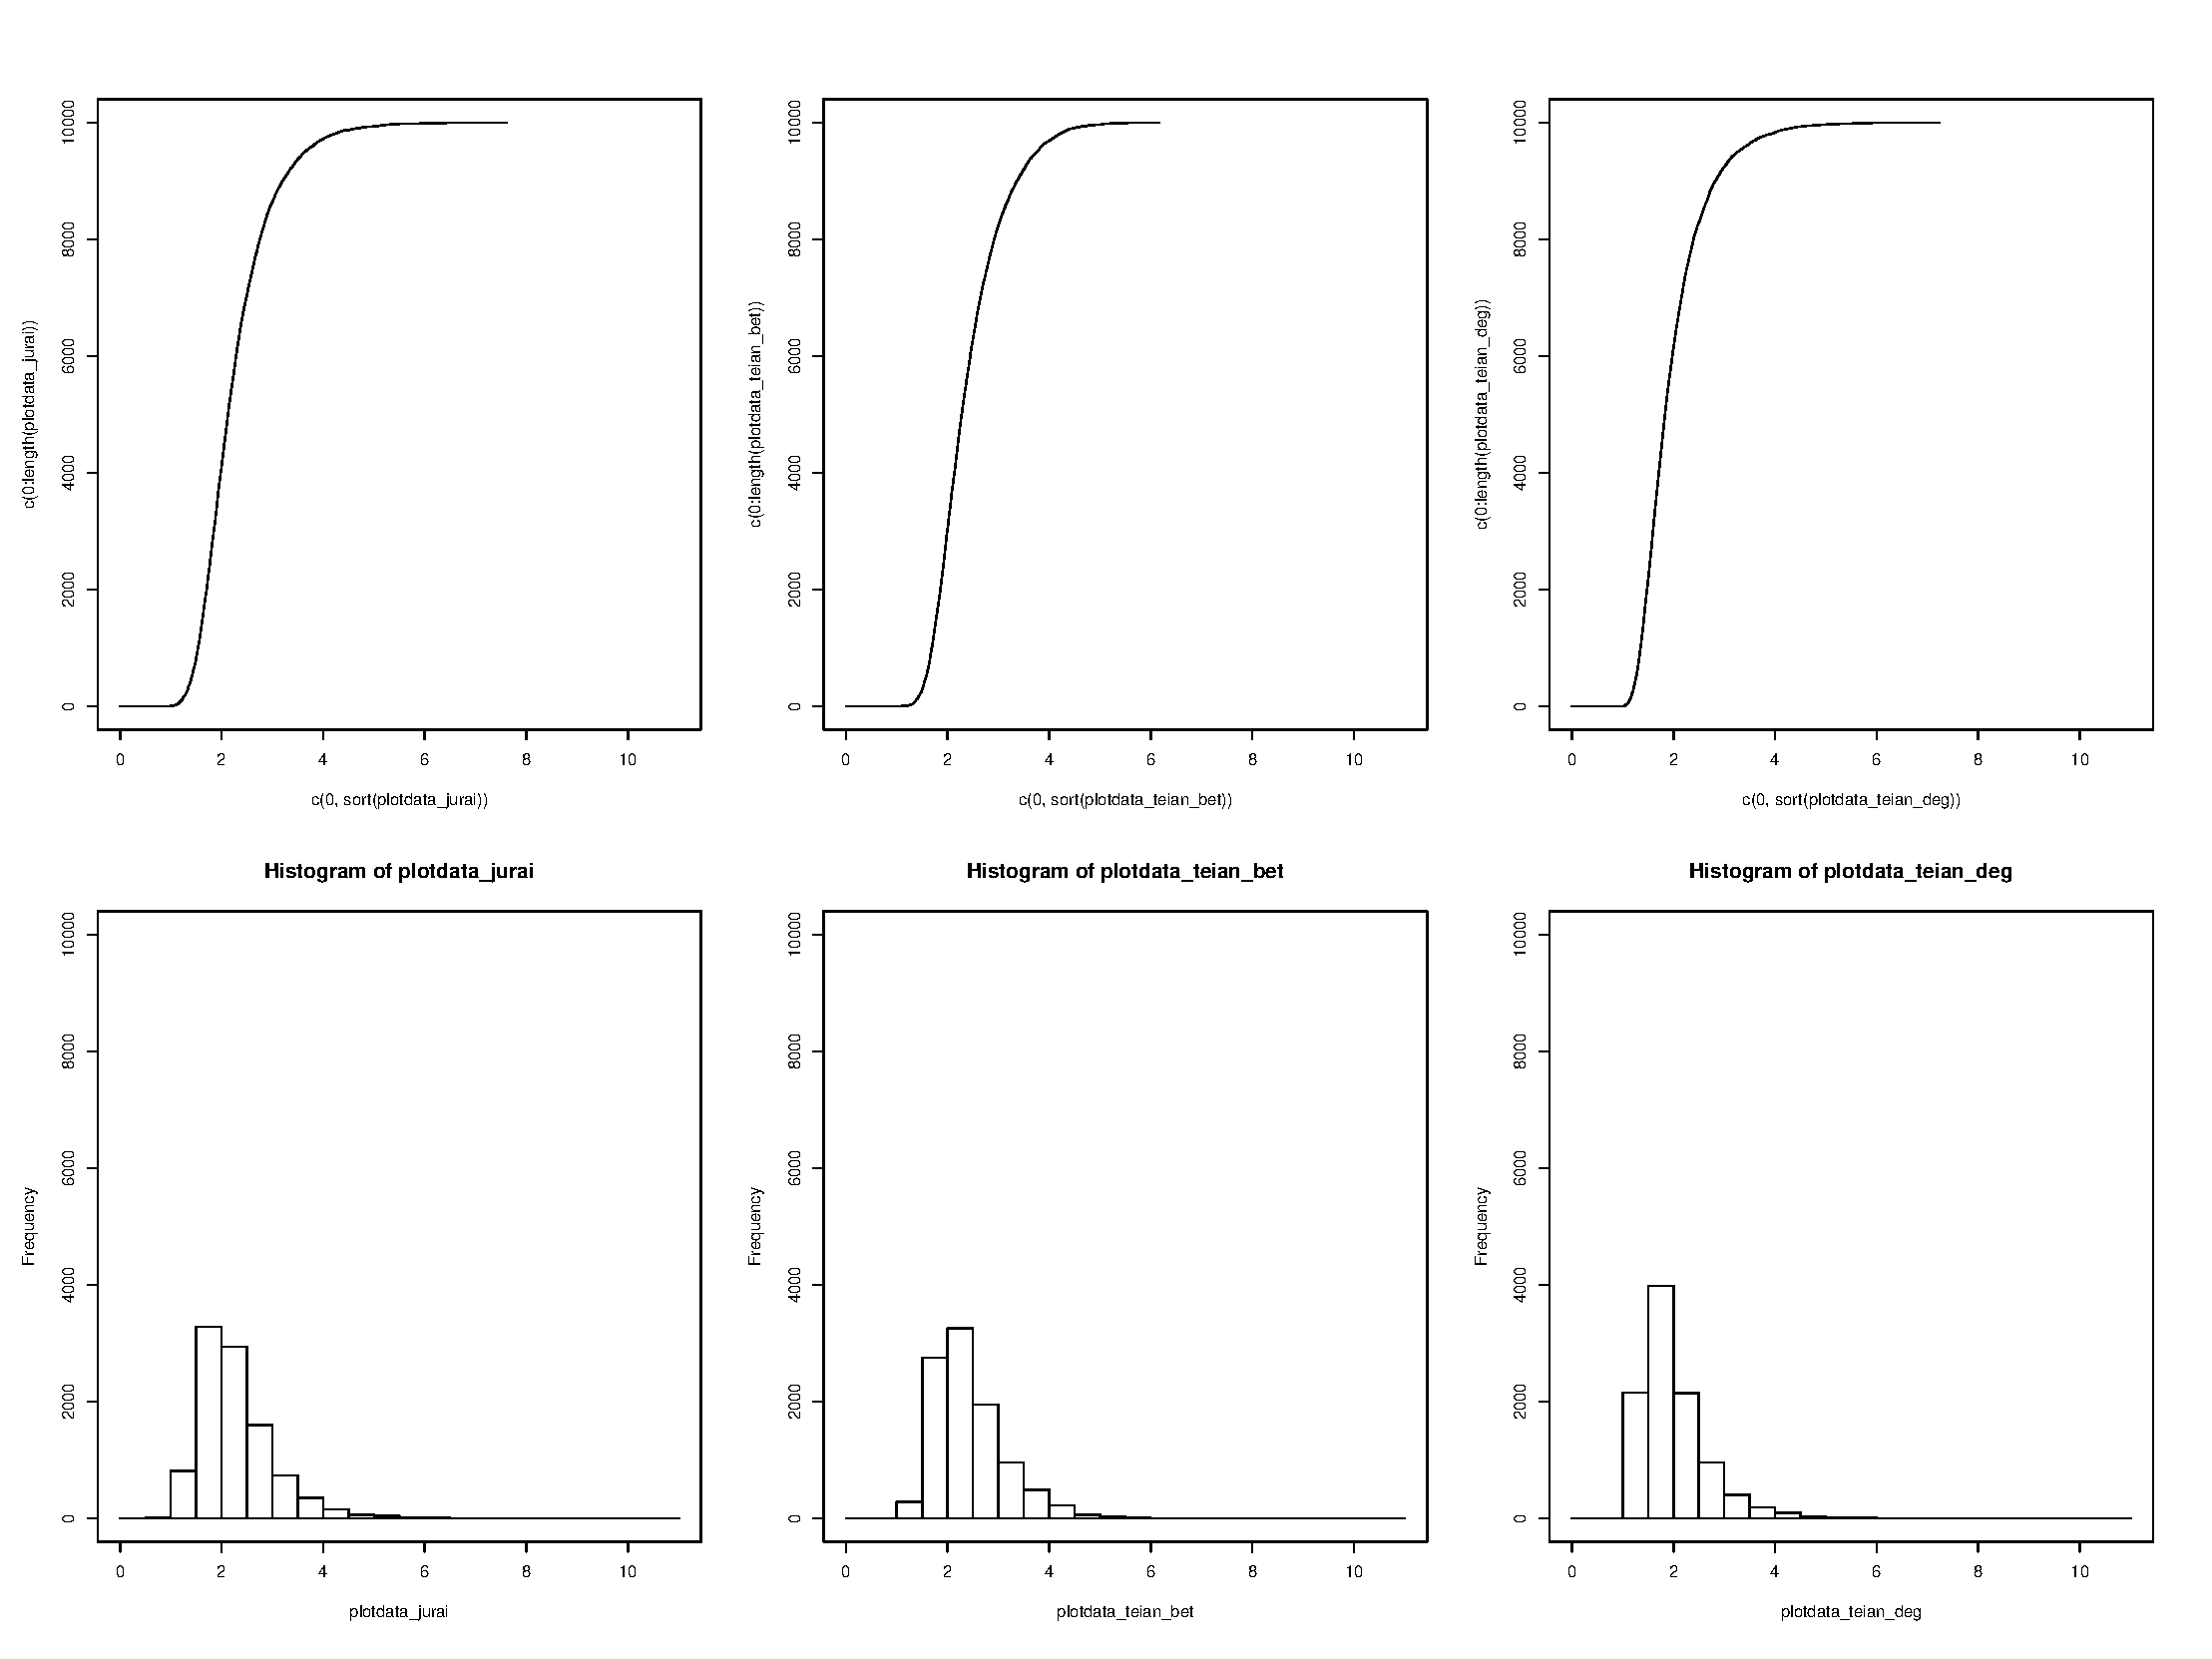
\includegraphics[width=1.2\textwidth]{figures/1_100_20.eps}
  \caption{方法1:100ノードで到達範囲を20としたとき}
  \label{fig:plot}
\end{figure}


\begin{figure}[H]
  \centering
  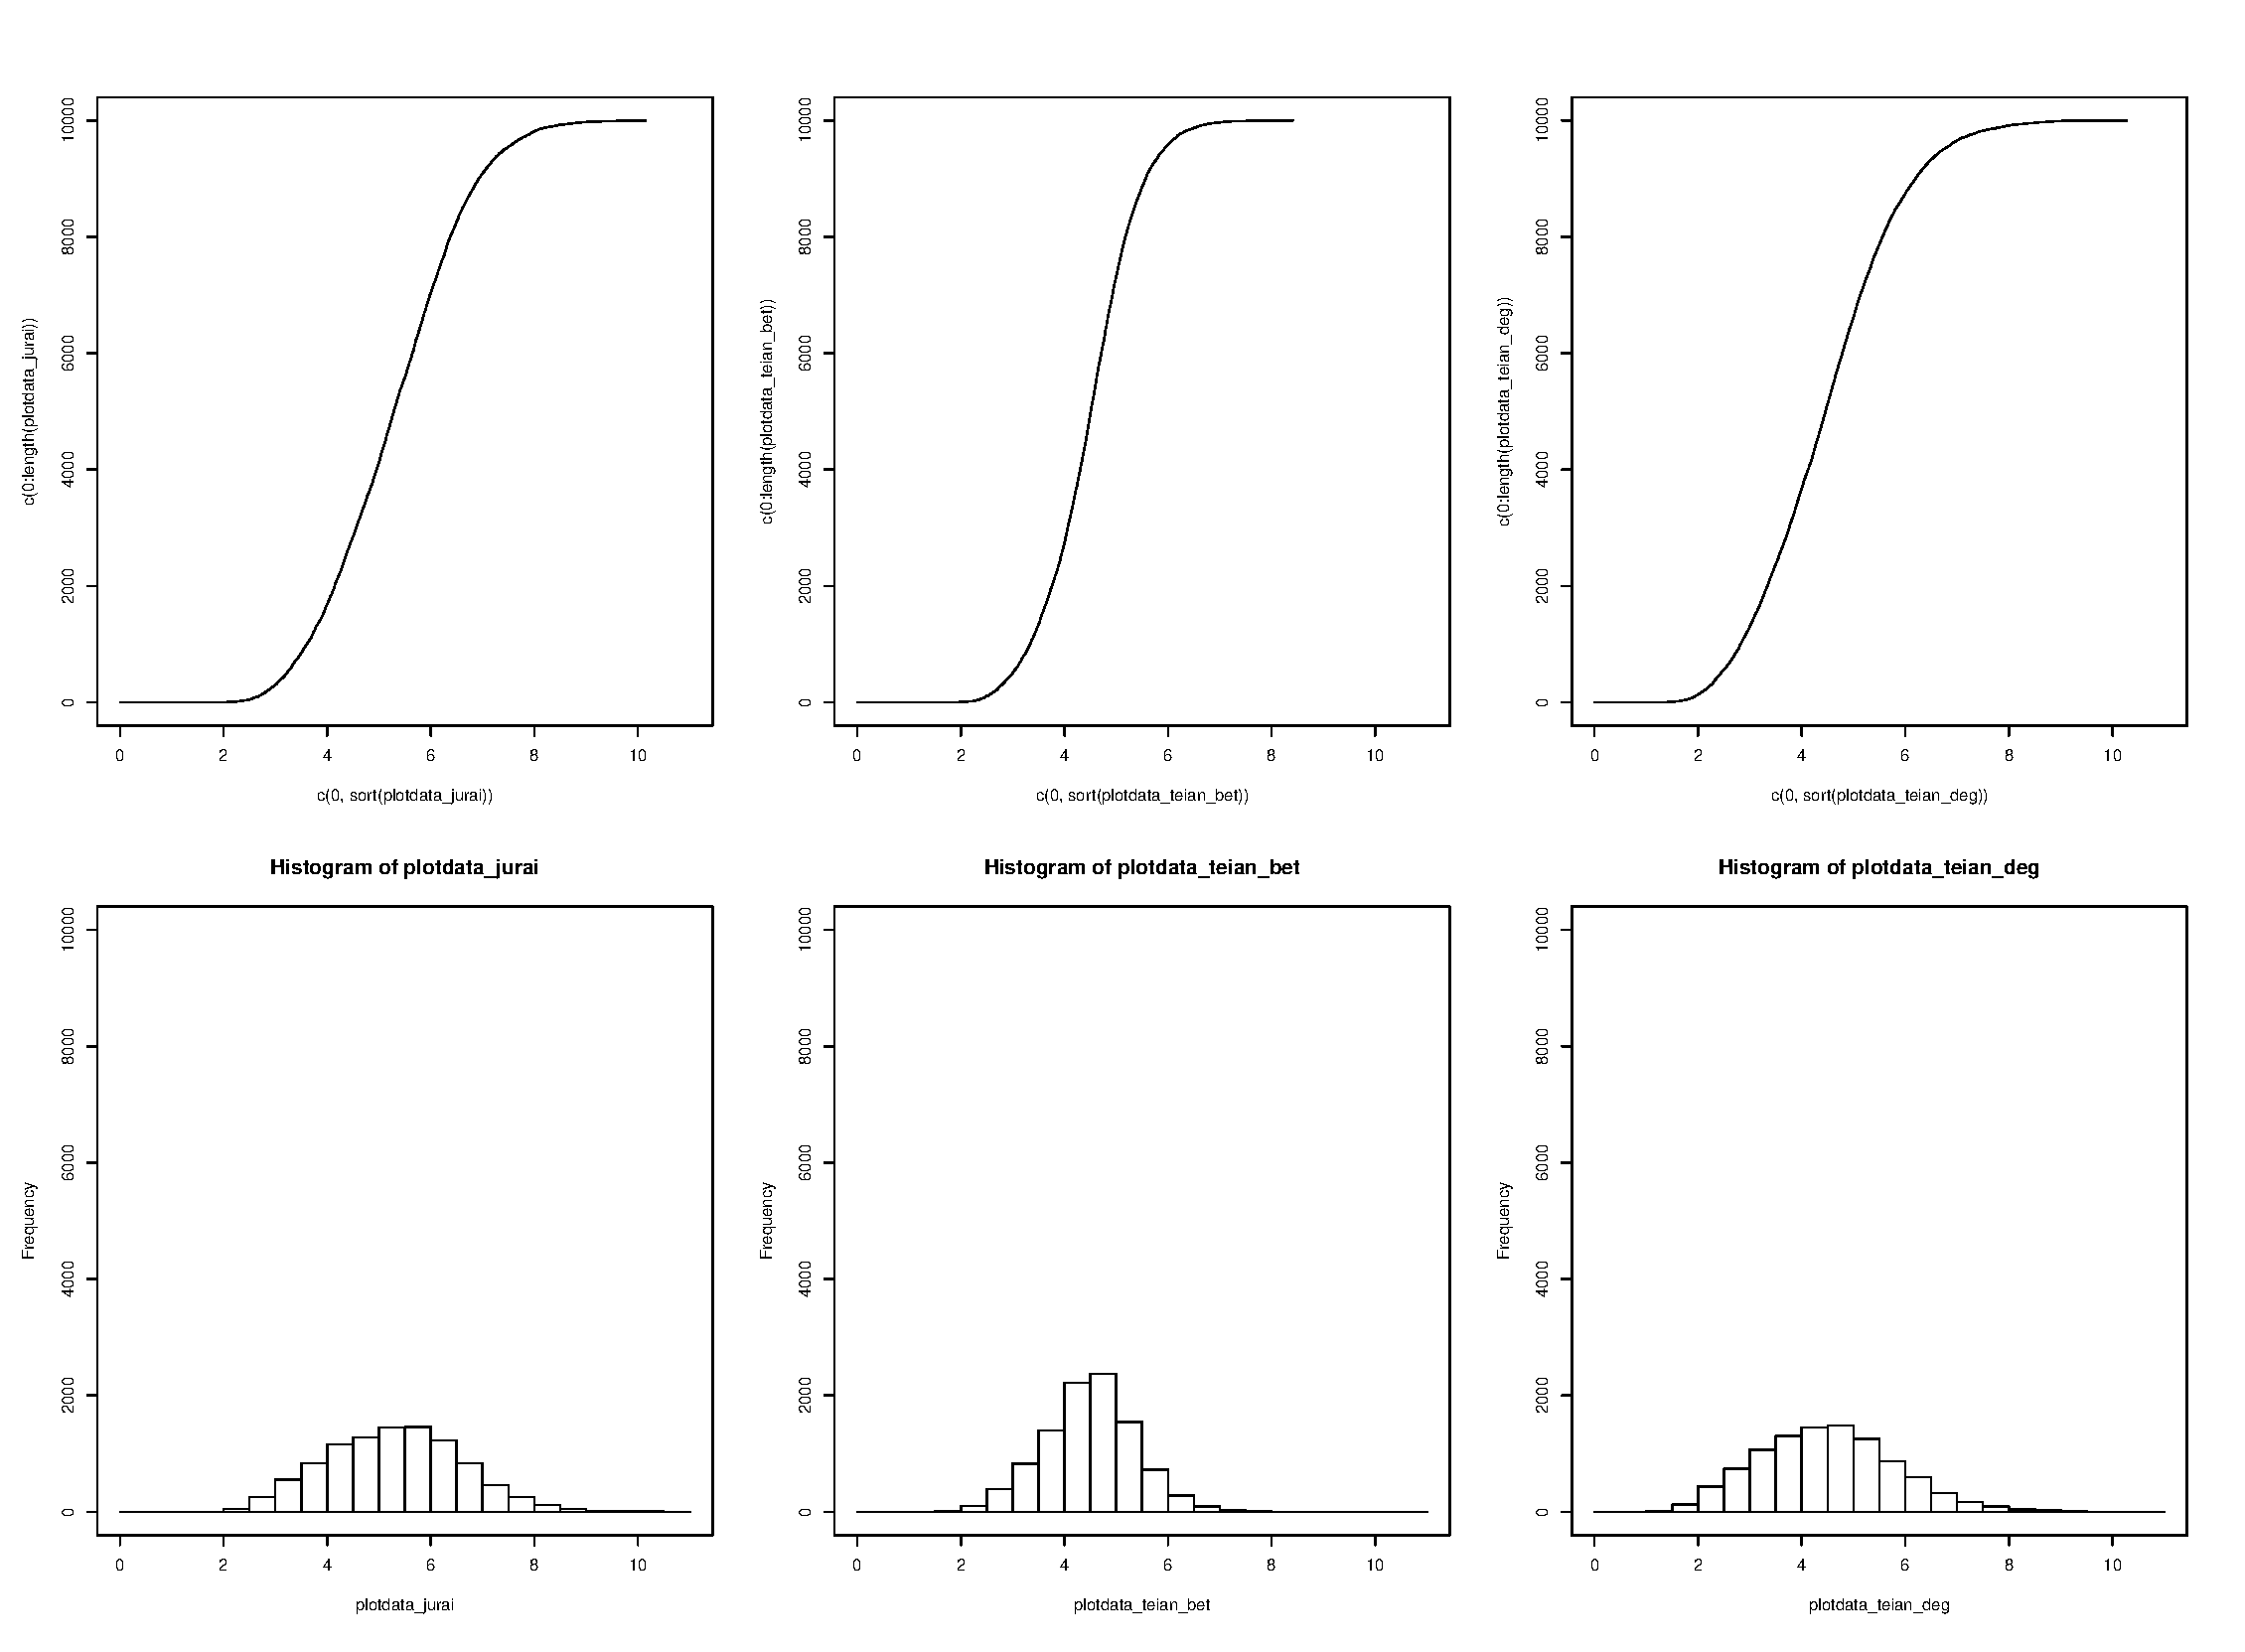
\includegraphics[width=1.2\textwidth]{figures/1_100_30.eps}
  \caption{方法1:100ノードで到達範囲を30としたとき}
  \label{fig:plot}
\end{figure}

\begin{figure}[H]
  \centering
  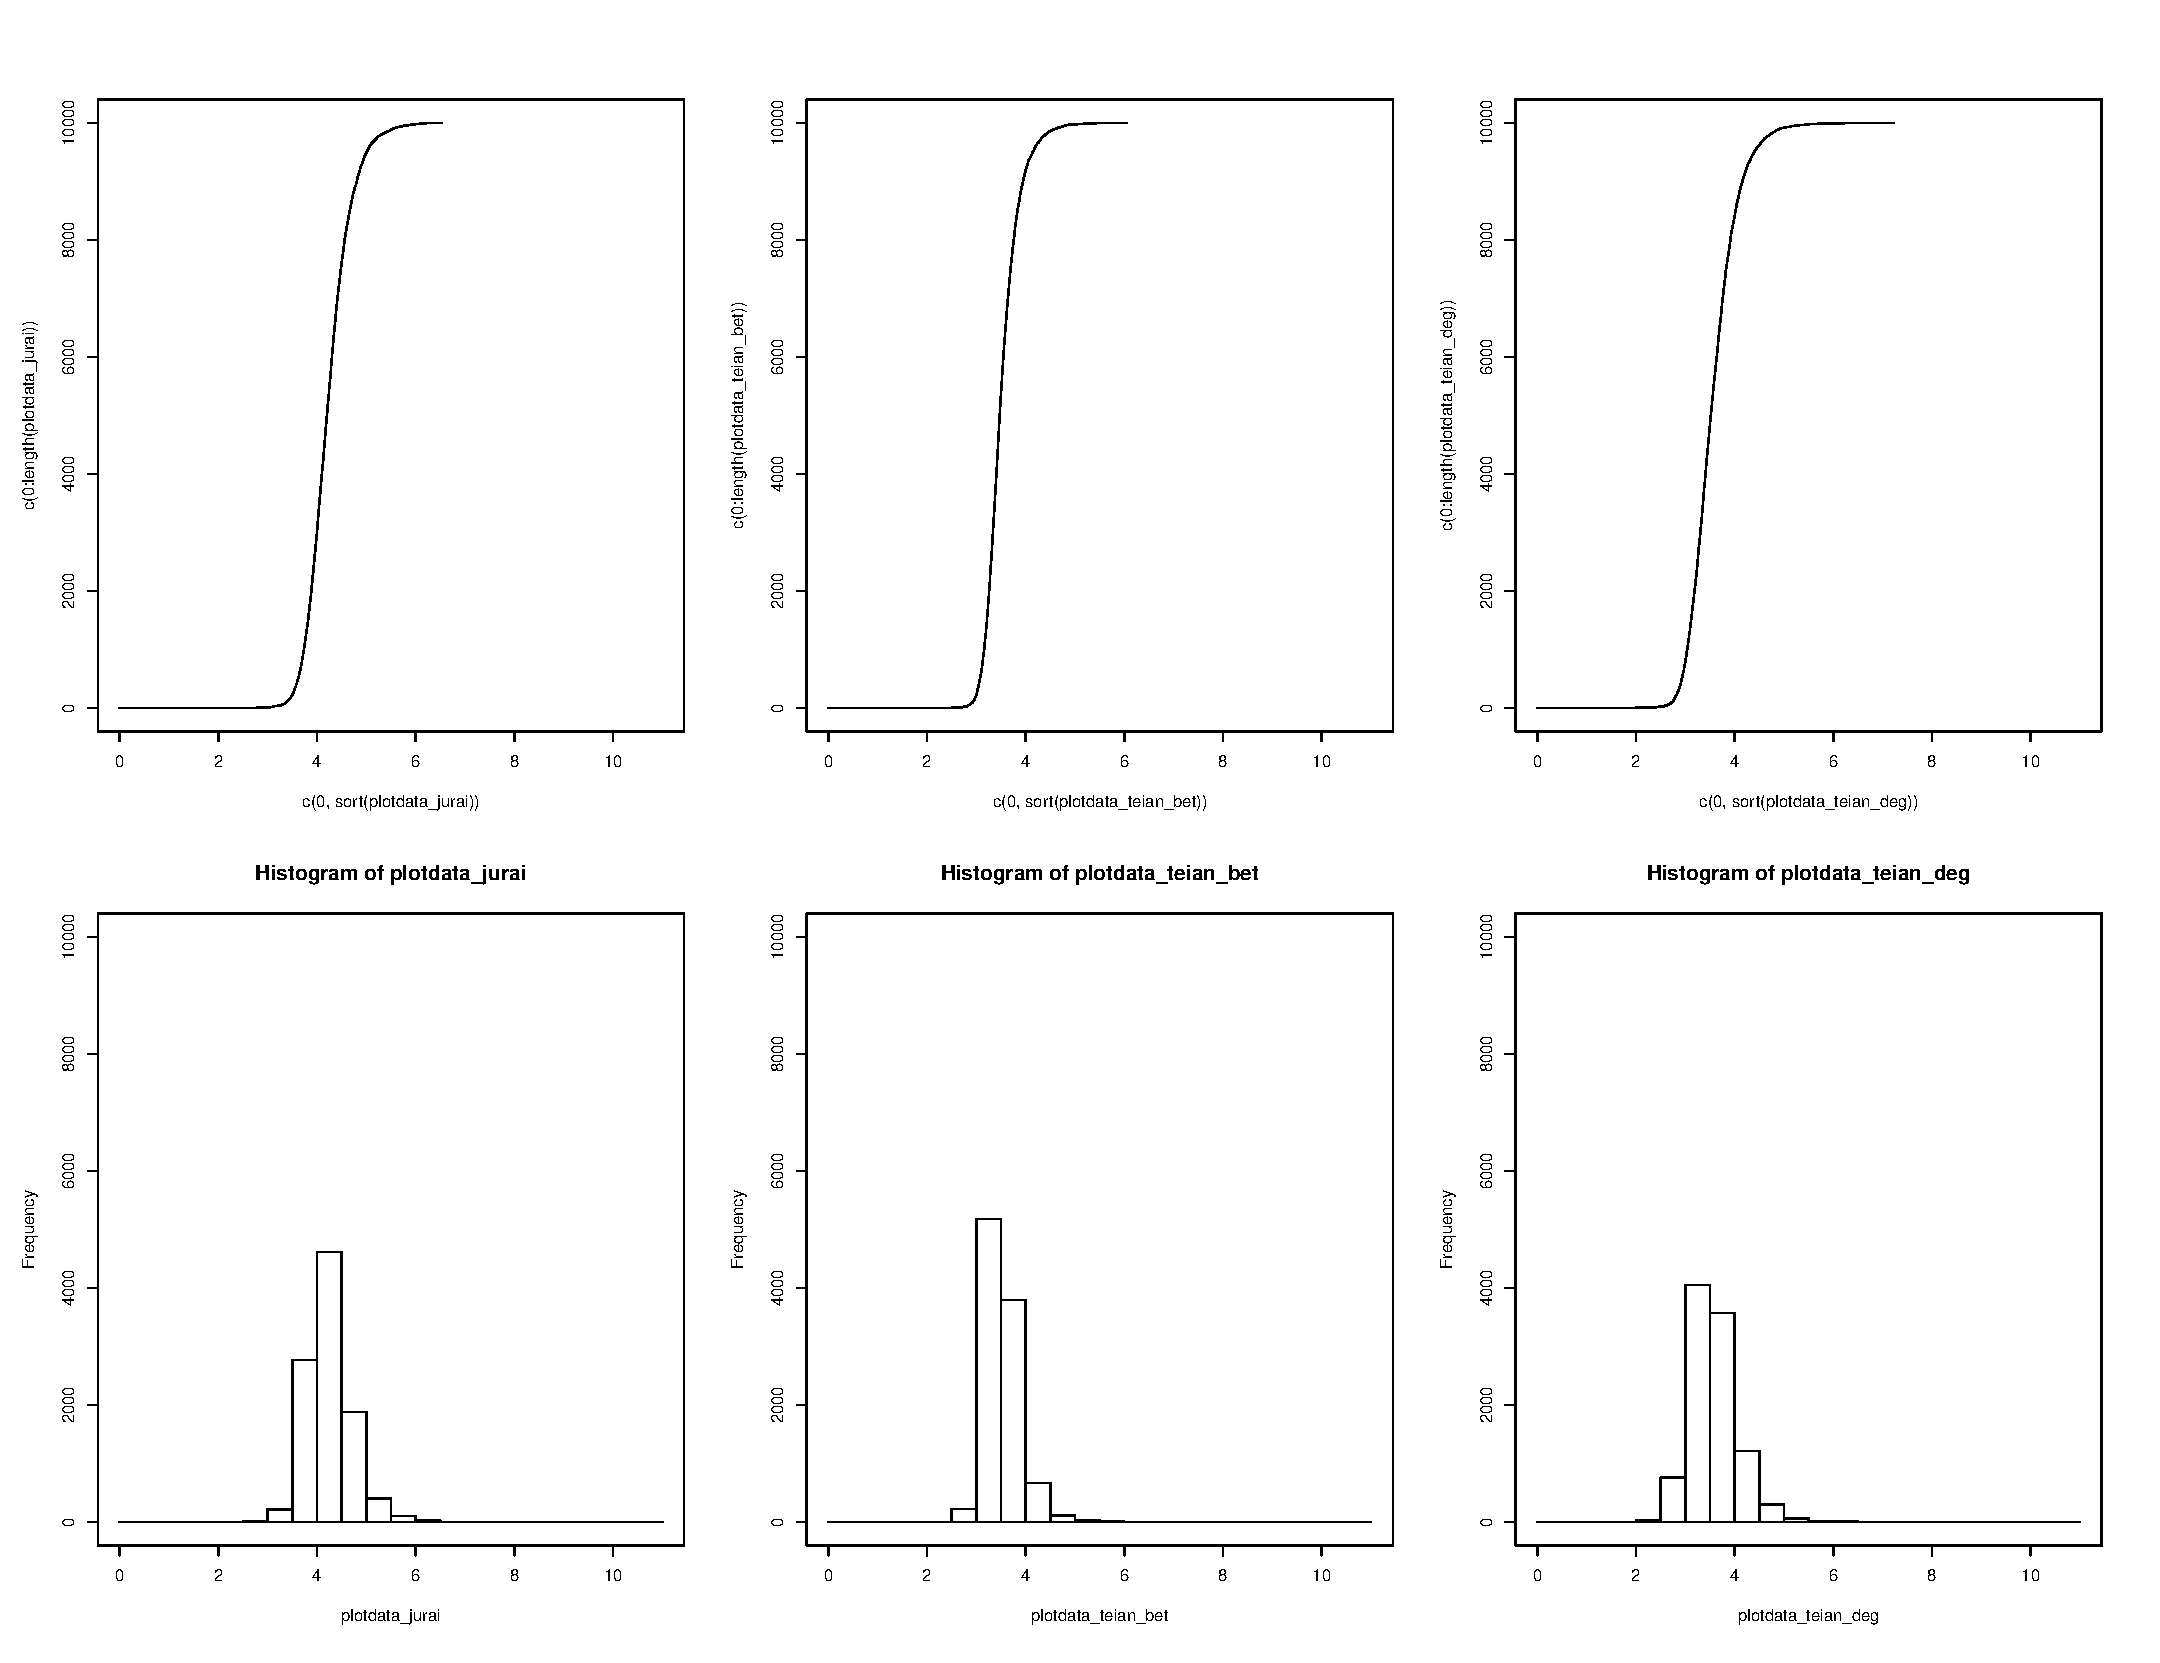
\includegraphics[width=1.2\textwidth]{figures/1_100_40.eps}
  \caption{方法1:100ノードで到達範囲を40としたとき}
  \label{fig:plot}
\end{figure}

\begin{figure}[H]
  \centering
  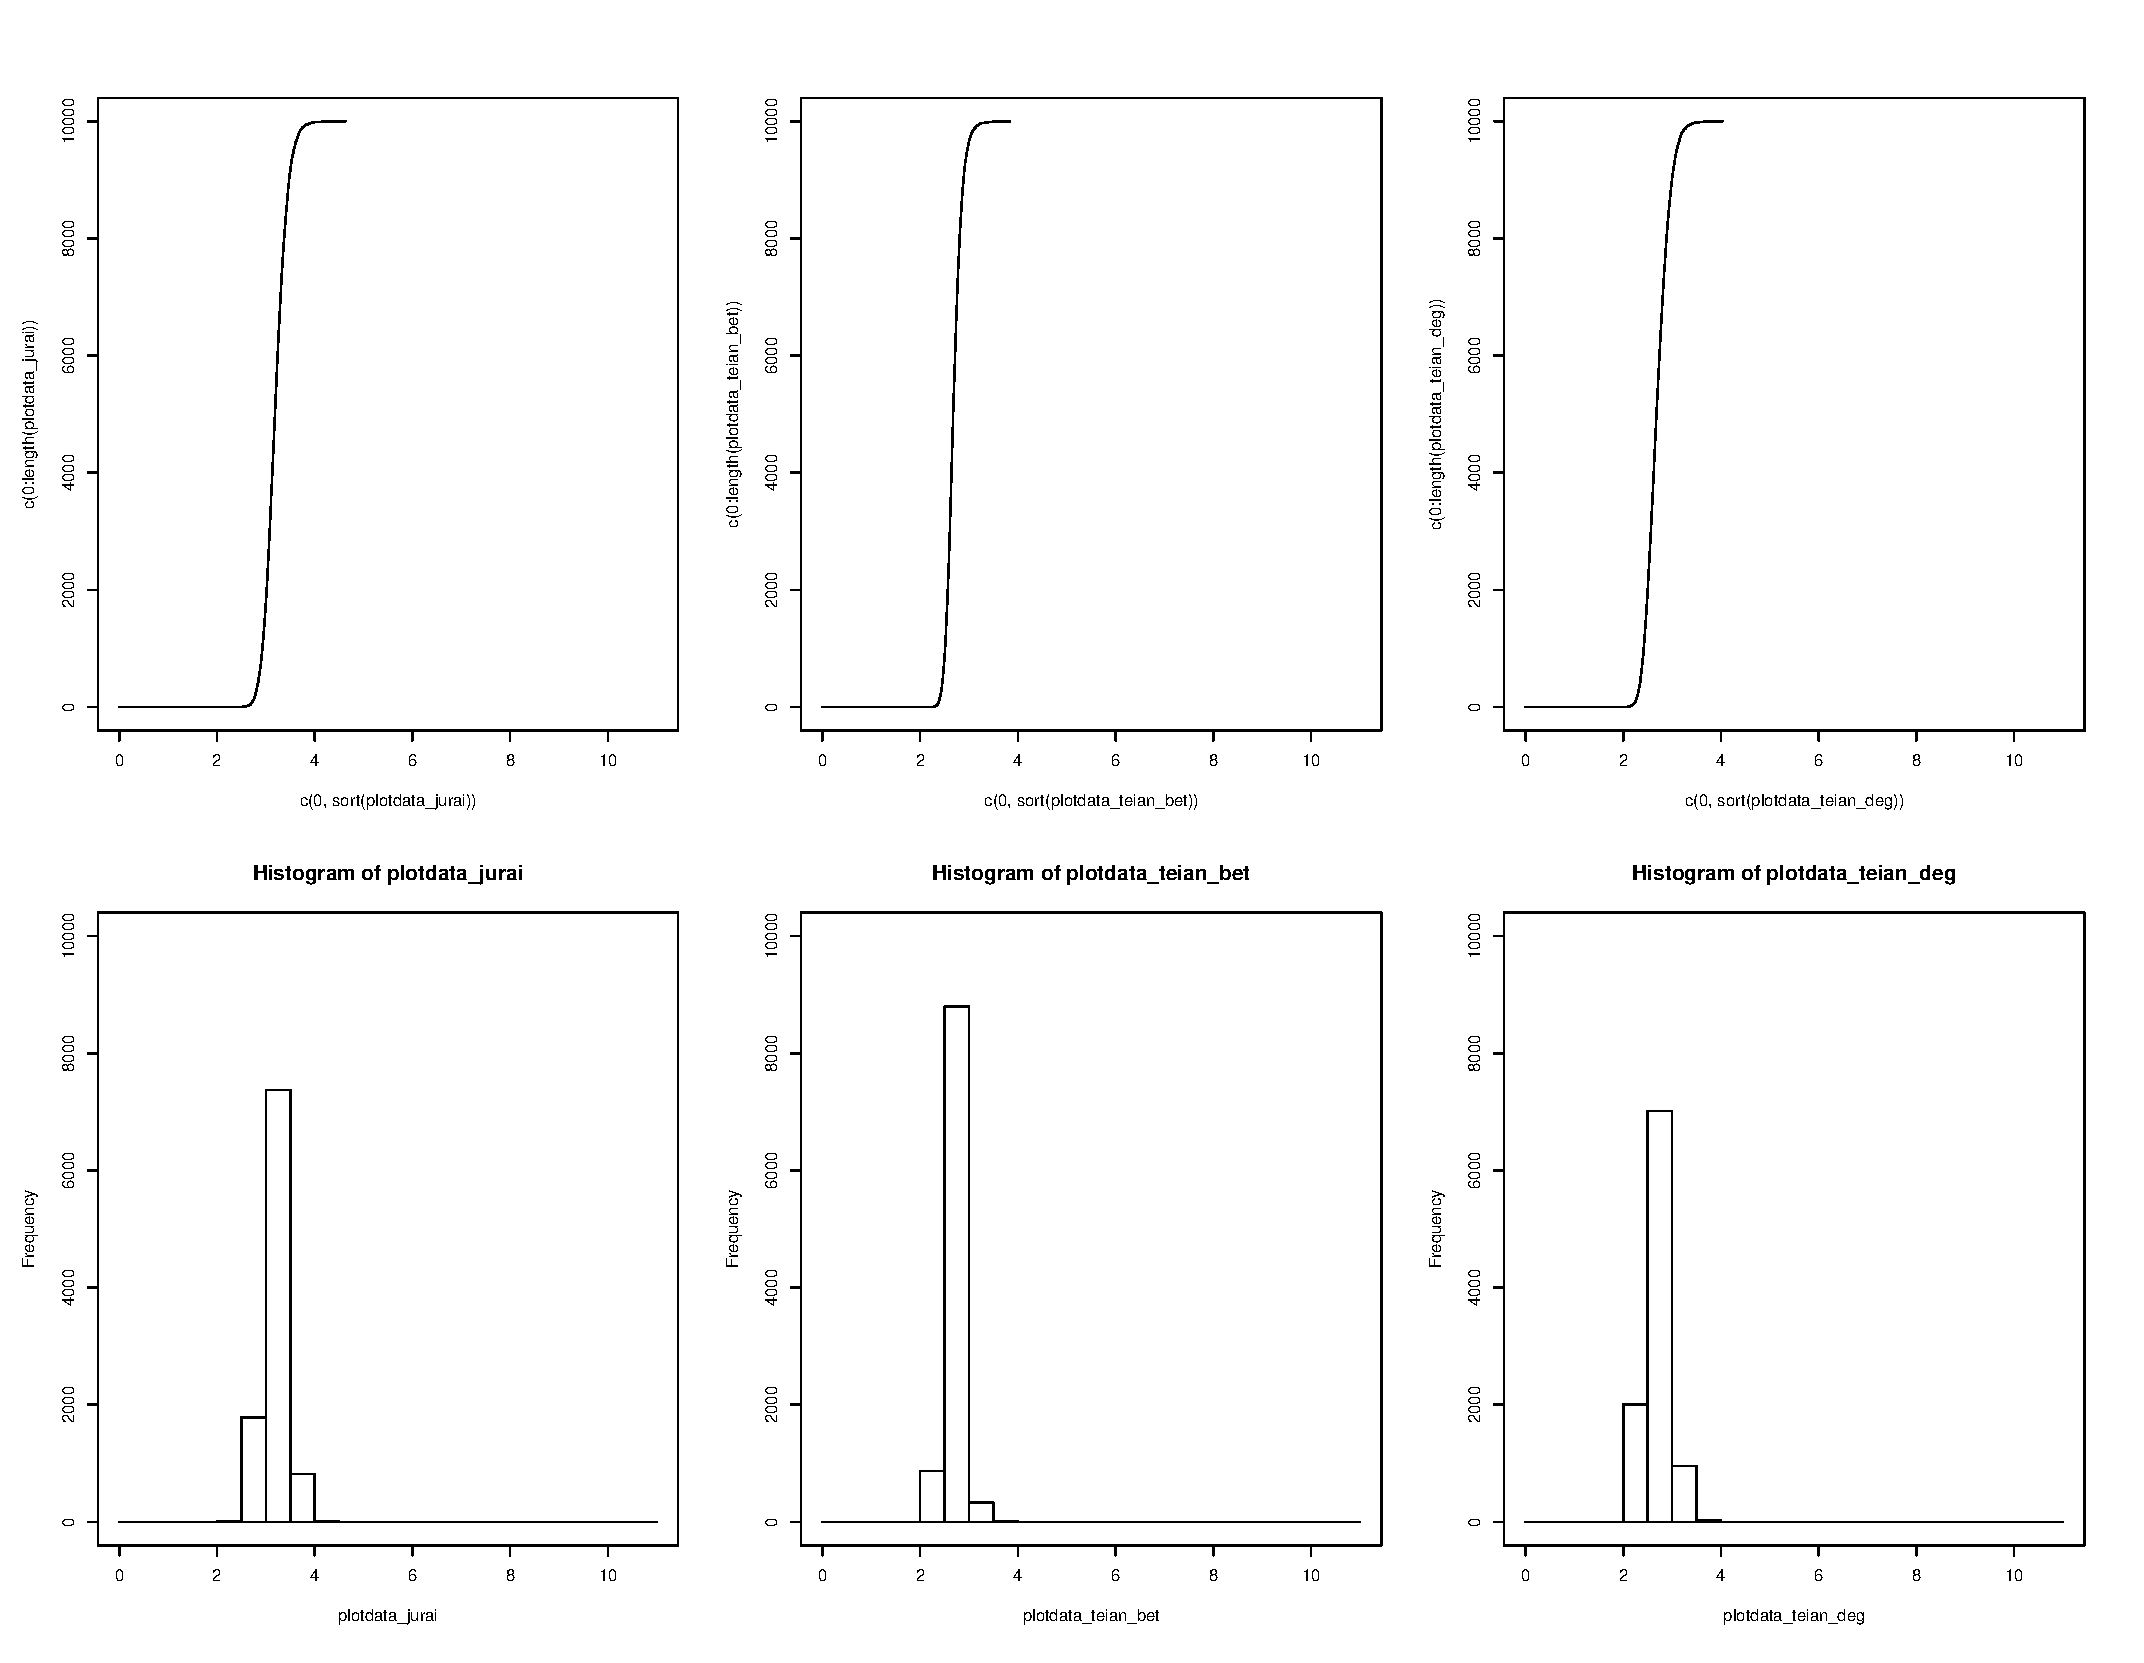
\includegraphics[width=1.2\textwidth]{figures/1_100_50.eps}
  \caption{方法1:100ノードで到達範囲を50としたとき}
  \label{fig:plot}
\end{figure}

\begin{figure}[H]
  \centering
  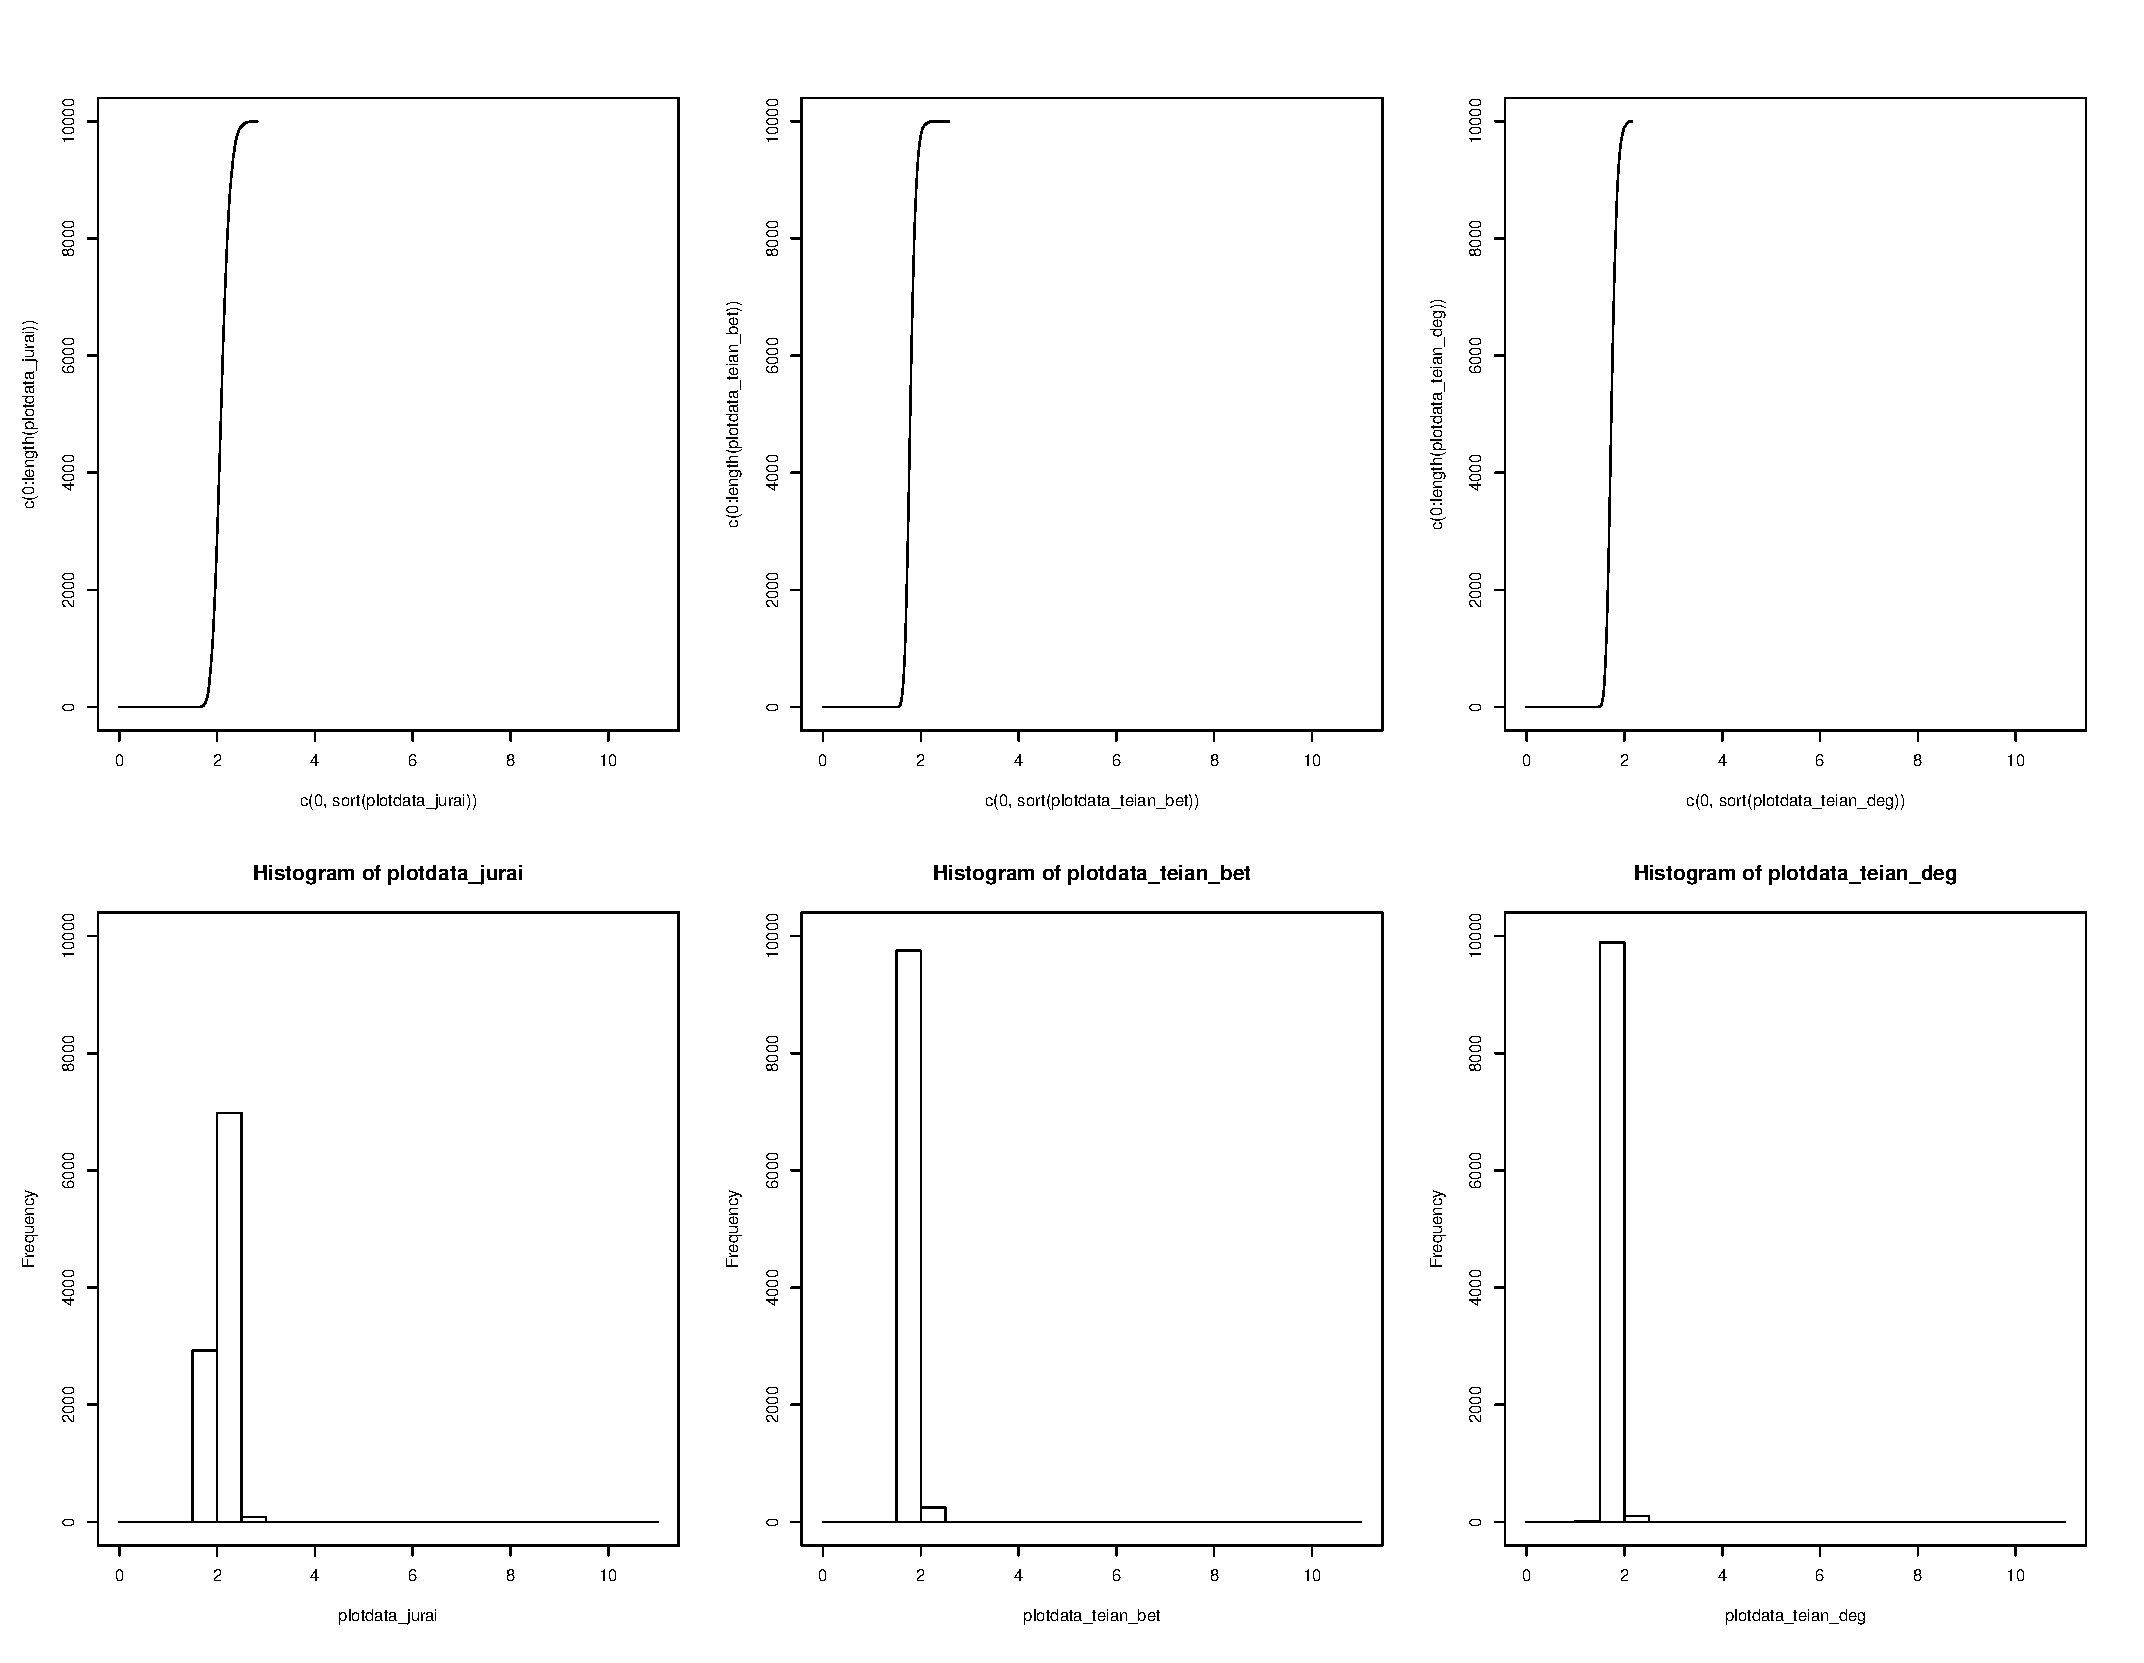
\includegraphics[width=1.2\textwidth]{figures/2_50.eps}
  \caption{方法2:50ノード}
  \label{fig:plot}
\end{figure}

\begin{figure}[H]
  \centering
  \includegraphics[width=1.2\textwidth]{figures/2_100.eps}
  \caption{方法2:100ノード}
  \label{fig:2_100}
\end{figure}
\end{landscape}

\chapter{結論と今後の課題}

\section{結論}
本研究では,同時送信フラッディングにおけるホスト選択がランダムにラウンドロビン方式で行われていることに着目し,ホストノードをネットワーク中心性に基づいて決定する手法を提案した.同時送信フラッディングのスケジューリングを担うホストノードと,他のノードにおいて,最短経路長平均の短縮とInf数が抑制されればより高信頼・低遅延な通信ができるのではと考えたからである.ホストノードをランダムに選出した場合と,中心性に基づき選出した場合でそれぞれ1万回ずつシミュレーションを行った.
その結果,最短経路長平均とInf数の両方において従来手法よりも提案手法の方が,優れていることがわかった.
2つの提案手法に関しては,最短経路長平均では,次数中心性によるホスト選択が優れていることがわかった.しかし,ノード密度があがるにつれ,従来手法と提案手法の最短経路長平均の差異はほとんどなくなった.つまり,ノードの密度が高い状況においてはホスト選択手法に関わらず最短経路長平均が短くなることがわかった.
一方,Inf数においては媒介中心性によるホスト選択が適していることがわかった.また,Inf数においてはノード密度が高くなっても従来手法と提案手法の差が縮まらなかった.これにより,ノードの密度に関わらず,ネットワーク分断を避けるためには提案手法が有効であることがわかった.
本研究では同時送信フラッディングにおける到達性を考慮したホスト選択に関して,媒介中心性によるホスト選択が優れているという結論になった.

まとめとして従来手法と提案手法2つの関係性を図\ref{tab:5_spl}と図\ref{tab:5_inf}に示す.

\begin{table}[H]
  \caption{最短経路長平均の結果}
  \begin{tabular}{c|c|c|c} \hline\hline
      &従来手法& 媒介中心性 & 次数中心性  \\ \hline 
    50 & × & △ & 〇\\
    100& △ & 〇 & 〇 \\\hline\hline
  \end{tabular}
  \label{tab:5_spl}
\end{table}

\begin{table}[H]
  \caption{Inf数の結果}
  \begin{tabular}{c|c|c|c} \hline\hline
      &従来手法& 媒介中心性 & 次数中心性  \\ \hline 
    50 & × & 〇 & △\\
    100 & × & 〇& △ \\\hline\hline
  \end{tabular}
  \label{tab:5_inf}
\end{table}



\section{今後の課題}

    (1)実装への課題\\
    本研究においては同時送信フラッディング前のメッセージ等の交換によってノード位置やネットワークトポロジを各ノードが把握している前提とした.この作業は従来手法では行われておらず,実装に当たってはそれぞれのノードにおけるホスト候補リストの整合性の確保が課題である.
    (2)他のネットワーク指標によるホスト選出\\
    ホスト選択指標として代表的なネットワーク指標である媒介中心性と次数中心性を用いることを提案したが,これ以外にもPageRankや近接中心性などの多くのネットワーク指標がある.こうしたネットワーク指標でもホスト選択を行い,比較する必要があると考える.
    (3)適切なホスト選択手法の選択\\
    本研究において,最短経路長平均とInf数で,適しているホスト選択手法が異なった.今後はネットワークの状況に応じて適切なホスト選択手法を選択できるとよいと考える,
    (4)ノード数を増やした検討\\
    本研究では,時間の都合上,50ノードと100ノードでシミュレーションを行い,提案手法の優位性を確認した.同時送信フラッディングを用いた構造モニタリングでは47台のセンサノードで900\si{\meter}の橋梁測定の実績があるが,今後ノード数を増やした場合においても提案手法が有効か検討が必要である.
    (5)実機での検討\\
    また,本研究においては距離のみに基づく到達判定によるシミュレーションを行ったため,実機や電波伝搬を考慮したシミュレーションによる検討が必要だと思われる.






\chapter*{謝辞}
初めに,指導教員である情報理工学域I\hspace{-1pt}I類セキュリティ情報学プログラムの山本嶺准教授の手厚いご指導に御礼申し上げます.常に相談しやすい雰囲気を作って下さり,私の至らない質問にも丁寧に答えてくださる姿勢が大変嬉しかったです.また,お忙しい中,私の教育実習の研究授業見学にも足を運んで下さいました.重ねて御礼申し上げます。

合同研究室の加藤聰彦教授や大坐畠智准教授には全体ゼミやシミュレーションゼミを通して適切なアドバイスをしていただき,研究を進める上で方向性を考えなおしたり,新しい視点をもつ機会を頂きました.ありがとうございました.

研究室の先輩方には,研究室生活や原稿の添削でお世話になりました。また,食事や鍋会を企画下さりありがとうございました.おかげさまで楽しい研究室生活を送れました. 

同期の皆様との雑談や他愛ない会話は,研究等がうまくいかないときの気分転換になり楽しかったです。1年間お世話になりました。

最後に,今日に至るまで何不自由ない暮らしをさせて下さった両親に感謝申し上げます。

\vspace{65mm}

\begin{flushright}
2020年2月6日(木)\\
情報理工学域I\hspace{-1pt}I類セキュリティ情報学プログラム\\
加藤山本研究室\\
4年 榎戸菜々穂
\end{flushright}

\bibliographystyle{sieicej}
\bibliography{ref.bib} 

\appendix



\end{document}
